% Options for packages loaded elsewhere
\PassOptionsToPackage{unicode}{hyperref}
\PassOptionsToPackage{hyphens}{url}
\PassOptionsToPackage{dvipsnames,svgnames,x11names}{xcolor}
%
\documentclass[
  11pt,
  a4paper,
]{article}

\usepackage{amsmath,amssymb}
\usepackage{iftex}
\ifPDFTeX
  \usepackage[T1]{fontenc}
  \usepackage[utf8]{inputenc}
  \usepackage{textcomp} % provide euro and other symbols
\else % if luatex or xetex
  \usepackage{unicode-math}
  \defaultfontfeatures{Scale=MatchLowercase}
  \defaultfontfeatures[\rmfamily]{Ligatures=TeX,Scale=1}
\fi
\usepackage{lmodern}
\ifPDFTeX\else  
    % xetex/luatex font selection
\fi
% Use upquote if available, for straight quotes in verbatim environments
\IfFileExists{upquote.sty}{\usepackage{upquote}}{}
\IfFileExists{microtype.sty}{% use microtype if available
  \usepackage[]{microtype}
  \UseMicrotypeSet[protrusion]{basicmath} % disable protrusion for tt fonts
}{}
\makeatletter
\@ifundefined{KOMAClassName}{% if non-KOMA class
  \IfFileExists{parskip.sty}{%
    \usepackage{parskip}
  }{% else
    \setlength{\parindent}{0pt}
    \setlength{\parskip}{6pt plus 2pt minus 1pt}}
}{% if KOMA class
  \KOMAoptions{parskip=half}}
\makeatother
\usepackage{xcolor}
\usepackage[margin=2.5cm]{geometry}
\setlength{\emergencystretch}{3em} % prevent overfull lines
\setcounter{secnumdepth}{5}
% Make \paragraph and \subparagraph free-standing
\ifx\paragraph\undefined\else
  \let\oldparagraph\paragraph
  \renewcommand{\paragraph}[1]{\oldparagraph{#1}\mbox{}}
\fi
\ifx\subparagraph\undefined\else
  \let\oldsubparagraph\subparagraph
  \renewcommand{\subparagraph}[1]{\oldsubparagraph{#1}\mbox{}}
\fi


\providecommand{\tightlist}{%
  \setlength{\itemsep}{0pt}\setlength{\parskip}{0pt}}\usepackage{longtable,booktabs,array}
\usepackage{calc} % for calculating minipage widths
% Correct order of tables after \paragraph or \subparagraph
\usepackage{etoolbox}
\makeatletter
\patchcmd\longtable{\par}{\if@noskipsec\mbox{}\fi\par}{}{}
\makeatother
% Allow footnotes in longtable head/foot
\IfFileExists{footnotehyper.sty}{\usepackage{footnotehyper}}{\usepackage{footnote}}
\makesavenoteenv{longtable}
\usepackage{graphicx}
\makeatletter
\def\maxwidth{\ifdim\Gin@nat@width>\linewidth\linewidth\else\Gin@nat@width\fi}
\def\maxheight{\ifdim\Gin@nat@height>\textheight\textheight\else\Gin@nat@height\fi}
\makeatother
% Scale images if necessary, so that they will not overflow the page
% margins by default, and it is still possible to overwrite the defaults
% using explicit options in \includegraphics[width, height, ...]{}
\setkeys{Gin}{width=\maxwidth,height=\maxheight,keepaspectratio}
% Set default figure placement to htbp
\makeatletter
\def\fps@figure{htbp}
\makeatother
% definitions for citeproc citations
\NewDocumentCommand\citeproctext{}{}
\NewDocumentCommand\citeproc{mm}{%
  \begingroup\def\citeproctext{#2}\cite{#1}\endgroup}
\makeatletter
 % allow citations to break across lines
 \let\@cite@ofmt\@firstofone
 % avoid brackets around text for \cite:
 \def\@biblabel#1{}
 \def\@cite#1#2{{#1\if@tempswa , #2\fi}}
\makeatother
\newlength{\cslhangindent}
\setlength{\cslhangindent}{1.5em}
\newlength{\csllabelwidth}
\setlength{\csllabelwidth}{3em}
\newenvironment{CSLReferences}[2] % #1 hanging-indent, #2 entry-spacing
 {\begin{list}{}{%
  \setlength{\itemindent}{0pt}
  \setlength{\leftmargin}{0pt}
  \setlength{\parsep}{0pt}
  % turn on hanging indent if param 1 is 1
  \ifodd #1
   \setlength{\leftmargin}{\cslhangindent}
   \setlength{\itemindent}{-1\cslhangindent}
  \fi
  % set entry spacing
  \setlength{\itemsep}{#2\baselineskip}}}
 {\end{list}}
\usepackage{calc}
\newcommand{\CSLBlock}[1]{\hfill\break\parbox[t]{\linewidth}{\strut\ignorespaces#1\strut}}
\newcommand{\CSLLeftMargin}[1]{\parbox[t]{\csllabelwidth}{\strut#1\strut}}
\newcommand{\CSLRightInline}[1]{\parbox[t]{\linewidth - \csllabelwidth}{\strut#1\strut}}
\newcommand{\CSLIndent}[1]{\hspace{\cslhangindent}#1}

\makeatletter
\@ifpackageloaded{caption}{}{\usepackage{caption}}
\AtBeginDocument{%
\ifdefined\contentsname
  \renewcommand*\contentsname{Table of contents}
\else
  \newcommand\contentsname{Table of contents}
\fi
\ifdefined\listfigurename
  \renewcommand*\listfigurename{List of Figures}
\else
  \newcommand\listfigurename{List of Figures}
\fi
\ifdefined\listtablename
  \renewcommand*\listtablename{List of Tables}
\else
  \newcommand\listtablename{List of Tables}
\fi
\ifdefined\figurename
  \renewcommand*\figurename{Figure}
\else
  \newcommand\figurename{Figure}
\fi
\ifdefined\tablename
  \renewcommand*\tablename{Table}
\else
  \newcommand\tablename{Table}
\fi
}
\@ifpackageloaded{float}{}{\usepackage{float}}
\floatstyle{ruled}
\@ifundefined{c@chapter}{\newfloat{codelisting}{h}{lop}}{\newfloat{codelisting}{h}{lop}[chapter]}
\floatname{codelisting}{Listing}
\newcommand*\listoflistings{\listof{codelisting}{List of Listings}}
\makeatother
\makeatletter
\makeatother
\makeatletter
\@ifpackageloaded{caption}{}{\usepackage{caption}}
\@ifpackageloaded{subcaption}{}{\usepackage{subcaption}}
\makeatother
\ifLuaTeX
  \usepackage{selnolig}  % disable illegal ligatures
\fi
\usepackage{bookmark}

\IfFileExists{xurl.sty}{\usepackage{xurl}}{} % add URL line breaks if available
\urlstyle{same} % disable monospaced font for URLs
\hypersetup{
  pdftitle={NBA and EuroLeague basketball, 2010/11--2025/26: a Bayesian replication and update},
  pdfauthor={Loukas Theodosiou},
  pdfkeywords={basketball, NBA, EuroLeague, Bayesian
statistics, replication, sports analytics},
  colorlinks=true,
  linkcolor={blue},
  filecolor={Maroon},
  citecolor={Blue},
  urlcolor={Blue},
  pdfcreator={LaTeX via pandoc}}

\title{NBA and EuroLeague basketball, 2010/11--2025/26: a Bayesian
replication and update}
\author{Loukas Theodosiou}
\date{2026-11-03}

\begin{document}
\maketitle
\begin{abstract}
Mandić and colleagues (2019) compared the NBA and the EuroLeague from
2000 to 2017 and concluded that the two leagues were becoming more
alike. We re-implement their model in Stan, reproduce all 68 of their
published estimates from their own data (largest difference 0.013), and
extend the comparison to sixteen seasons (2010/11--2025/26), 24,874
games and 4,057,782 located shots. Bayesian mixed models with team- and
opponent-season effects describe the leagues today; second-order
random-walk trends, a shift model with a discrete lag and a ``time gap''
estimate describe how they changed; a matched design compares playoffs
with the same teams' regular seasons; and shrinkage style profiles place
every team and player on its league's path through time. Today the two
leagues shoot equally well and take the same share of their shots from
three (41.1\% in both), but they differ in style: the NBA plays 10.4
more possessions per 40 minutes and the EuroLeague commits 7.5 more
fouls per 100 possessions. Shot mix converged while pace diverged. On
three-point shooting the EuroLeague moves with the NBA or a season
behind it; on volume measures it resembles the NBA of three to five
seasons ago. Houston (NBA) and Real Madrid (EuroLeague) played their
leagues' future most clearly. Code, models and figures are openly
available.
\end{abstract}

\section{Introduction}\label{introduction}

The NBA and the EuroLeague are the two strongest basketball competitions
in the world, but they are played under different rules (a 48- against a
40-minute game, a 7.24 m against a 6.75 m three-point line, different
defensive and foul rules) and by teams built in different ways. How the
two leagues differ, and whether they are becoming alike, matters to
coaches and scouts who move players between them and to analysts who
compare their statistics.

Mandić et al. (2019) compared the leagues from 2000/01 to 2016/17 with a
Bayesian model of season means and linear trends. They found that the
NBA was moving towards the EuroLeague's style, most clearly in
three-point shooting, and that NBA playoff basketball looked more
``European'' than the NBA's regular season. Since 2017 the three-point
revolution has continued (Goldsberry 2019), both leagues have changed
rules (the 14-second shot-clock reset after an offensive rebound reached
the NBA in 2018/19), and shot-location data have become available for
both leagues, which allows comparisons the original box-score study
could not make (Erčulj and Štrumbelj 2015).

This paper replicates and extends that study. We ask four questions:

\begin{itemize}
\tightlist
\item
  \textbf{RQ1.} How do the two leagues differ today (2023/24--2025/26),
  in box scores and in where shots are taken and made?
\item
  \textbf{RQ2.} How have they changed since 2010/11? Are they
  converging, and does one league follow the other?
\item
  \textbf{RQ3.} How does play change in the playoffs, and do NBA
  playoffs look more like the EuroLeague?
\item
  \textbf{RQ4.} Which teams and players embodied their league's typical
  style, and which were ahead of their time?
\end{itemize}

The contributions are (i) a full replication of the 2019 model on the
authors' own data; (ii) an update to 2025/26 with models that separate
team, opponent and season effects; (iii) new analyses of convergence,
lead--lag and playoff change; and (iv) a probabilistic ``time position''
for every team and player. All code, models and figures are open.

\section{Data}\label{data}

Box scores come from ESPN for the NBA, through the hoopR package (Gilani
2021), and from the official EuroLeague API for the EuroLeague. Shot
locations come from NBA Stats (through hoopR) and from the EuroLeague
API. The main window is 2010/11--2025/26: 24,874 games and 4,057,782
field-goal attempts with court coordinates. Seasons from 2001/02 are
used only for the lead--lag model. Seasons are labelled by their
starting year in the code (2010 = 2010/11).

The metrics follow Mandić et al. (2019) exactly. Possessions are 2PA +
3PA + 0.5·FTA + TOV; counting statistics are per 100 possessions; the
four factors (Oliver 2004; Kubatko et al. 2007) are computed for each
team and its opponent; free throws are counted per foul received; and
rotation depth is the entropy of minutes played. We add possessions per
40 minutes (to put the 48- and 40-minute games on one scale), points per
100 possessions and the share of field-goal attempts taken from three.

\textbf{Two scorekeeping systems.} Rebounds and turnovers are summed
over players in both leagues, because team rebounds and team turnovers
are recorded differently. EuroLeague scorers place layups and dunks
about 1.1 m from the hoop on average, so close-range EuroLeague shots
appear as a ring rather than at the rim; the rim area is therefore
defined as within 1.75 m. Shots are grouped into five zones: rim area
(\textless{} 1.75 m), short mid-range (1.75--4.25 m), long mid-range
(two-pointers beyond 4.25 m), corner three and above-the-break three,
each with its own league's court geometry.

\textbf{Playoffs.} NBA playoffs exclude the play-in. EuroLeague playoffs
are the playoff series and the Final Four; the former Top 16 counts as
regular season (the 2019 paper counted it as playoffs) and the 2025/26
play-in is dropped.

\section{Methods}\label{methods}

All models are Bayesian and fitted in Stan (Carpenter et al. 2017),
directly or through brms (Bürkner 2017). Every reported model passed the
usual checks (R-hat ≤ 1.04, no or negligible divergent transitions).
Figures were drawn with the ggbasket package (Theodosiou 2026).

\textbf{Replication (RQ2).} The 2019 model describes each league and
metric by game-level values \(y_{ij} \sim N(\mu_j, \sigma_j)\) in season
\(j\), with season means on a line,
\(\mu_j \sim N(\mu + s\,t_j, \sigma)\), and flat priors. Because games
are independent and normal within a season, the season's game count,
mean and variance are sufficient statistics; we write the model on them,
which gives the same posterior about a thousand times faster. Fitted to
the authors' published data (PLOS ONE S1 Data), it reproduces their
Table 1 (Section~\ref{sec-replication}).

\textbf{Differences today (RQ1).} Each metric is standardised and
modelled at team-game level as
\(z \sim N(\beta_{\text{league}} + u_{\text{team-season}} + v_{\text{opponent-season}},
\sigma_{\text{league}})\), with weakly informative priors (\(N(0, 1.5)\)
on league effects, \(N(0, 1)\) on standard deviations). The league
difference is reported in game-to-game standard deviations and on the
original scale. Shot shares and accuracy by zone use binomial models
with team-season effects; accuracy across the court uses a binomial
model with a smooth two-dimensional tensor-product surface per league
(Wood 2017).

\textbf{Trends and convergence (RQ2).} Season means are modelled as a
second-order random walk (RW2) (Rue and Held 2005) plus season-specific
shocks, \(\bar y_t \sim N(f_t, \sqrt{se_t^2 + \tau^2})\) with
\(f_t = 2f_{t-1} - f_{t-2} + \omega\,\varepsilon_t\). When
\(\omega \to 0\) the trend is the straight line of the 2019 model.
Because all terms are Gaussian, the curve is integrated out analytically
and only \(\omega\) and \(\tau\) are sampled; curves are then drawn from
their exact conditional distribution. The gap between the leagues'
curves, and the probability that it shrank, follow from the joint draws.

\textbf{Lead--lag (RQ2).} A shift model asks whether the EuroLeague's
trend equals the NBA's shifted by \(k\) seasons,
\(\bar y^{E}_t \sim N(a + b\,f_{t-k}, \cdot)\), with
\(k \in \{-5, \dots, 5\}\) marginalised out, so the posterior
\(P(k \mid \text{data})\) says how strongly each lag is supported.
Probability that piles up at the edges of the window means that no lag
fits well. A second, descriptive measure finds, for each posterior draw
of the NBA curve, the season in which the NBA first reached the
EuroLeague's 2025/26 level (``time gap'').

\textbf{Playoffs (RQ3).} Only teams that reached the playoffs are used,
each compared with its own regular season, with team- and
opponent-season effects:
\(z \sim N(\beta_{\text{league}} + \gamma_{\text{league}}\cdot\text{playoff} + u + v, \sigma)\).
For each metric we also compute the probability that the NBA's playoff
shift points towards the EuroLeague's regular-season level.

\textbf{Style profiles (RQ4).} Each team-season is described by 14
numbers (pace, five-zone shot mix, free throws, assists, turnovers,
offensive rebounds, blocks, steals, fouls and rotation depth) and each
rotation player-season by 13, always compared with players of the same
position. Profiles are conjugate posteriors (Dirichlet--multinomial for
shot mix, gamma--Poisson for rates, normal for game means) with prior
strength estimated by marginal likelihood (empirical Bayes), so small
samples are shrunk towards the league--season average. A team's
\emph{time position} is the season on its league's path through style
space that it is closest to; a team of 2012/13 closest to the league of
2016/17 is four seasons ahead.

\section{Results}\label{results}

\subsection{How the leagues differ today
(RQ1)}\label{how-the-leagues-differ-today-rq1}

The two leagues now shoot alike (Figure~\ref{fig-box}). Three-point
percentage (36.1\% NBA, 36.1\% EuroLeague), free-throw percentage,
effective field-goal percentage and the share of shots taken from three
(41.1\% against 41.1\%) are practically identical. They differ in style.
The NBA plays faster (94.2 against 83.8 possessions per 40 minutes),
blocks more and earns more free throws per foul (1.16 against 0.90). The
EuroLeague fouls far more (24.3 against 16.8 per 100 possessions), turns
the ball over more and rebounds more of its own misses.

\begin{figure}[htbp]

\centering{

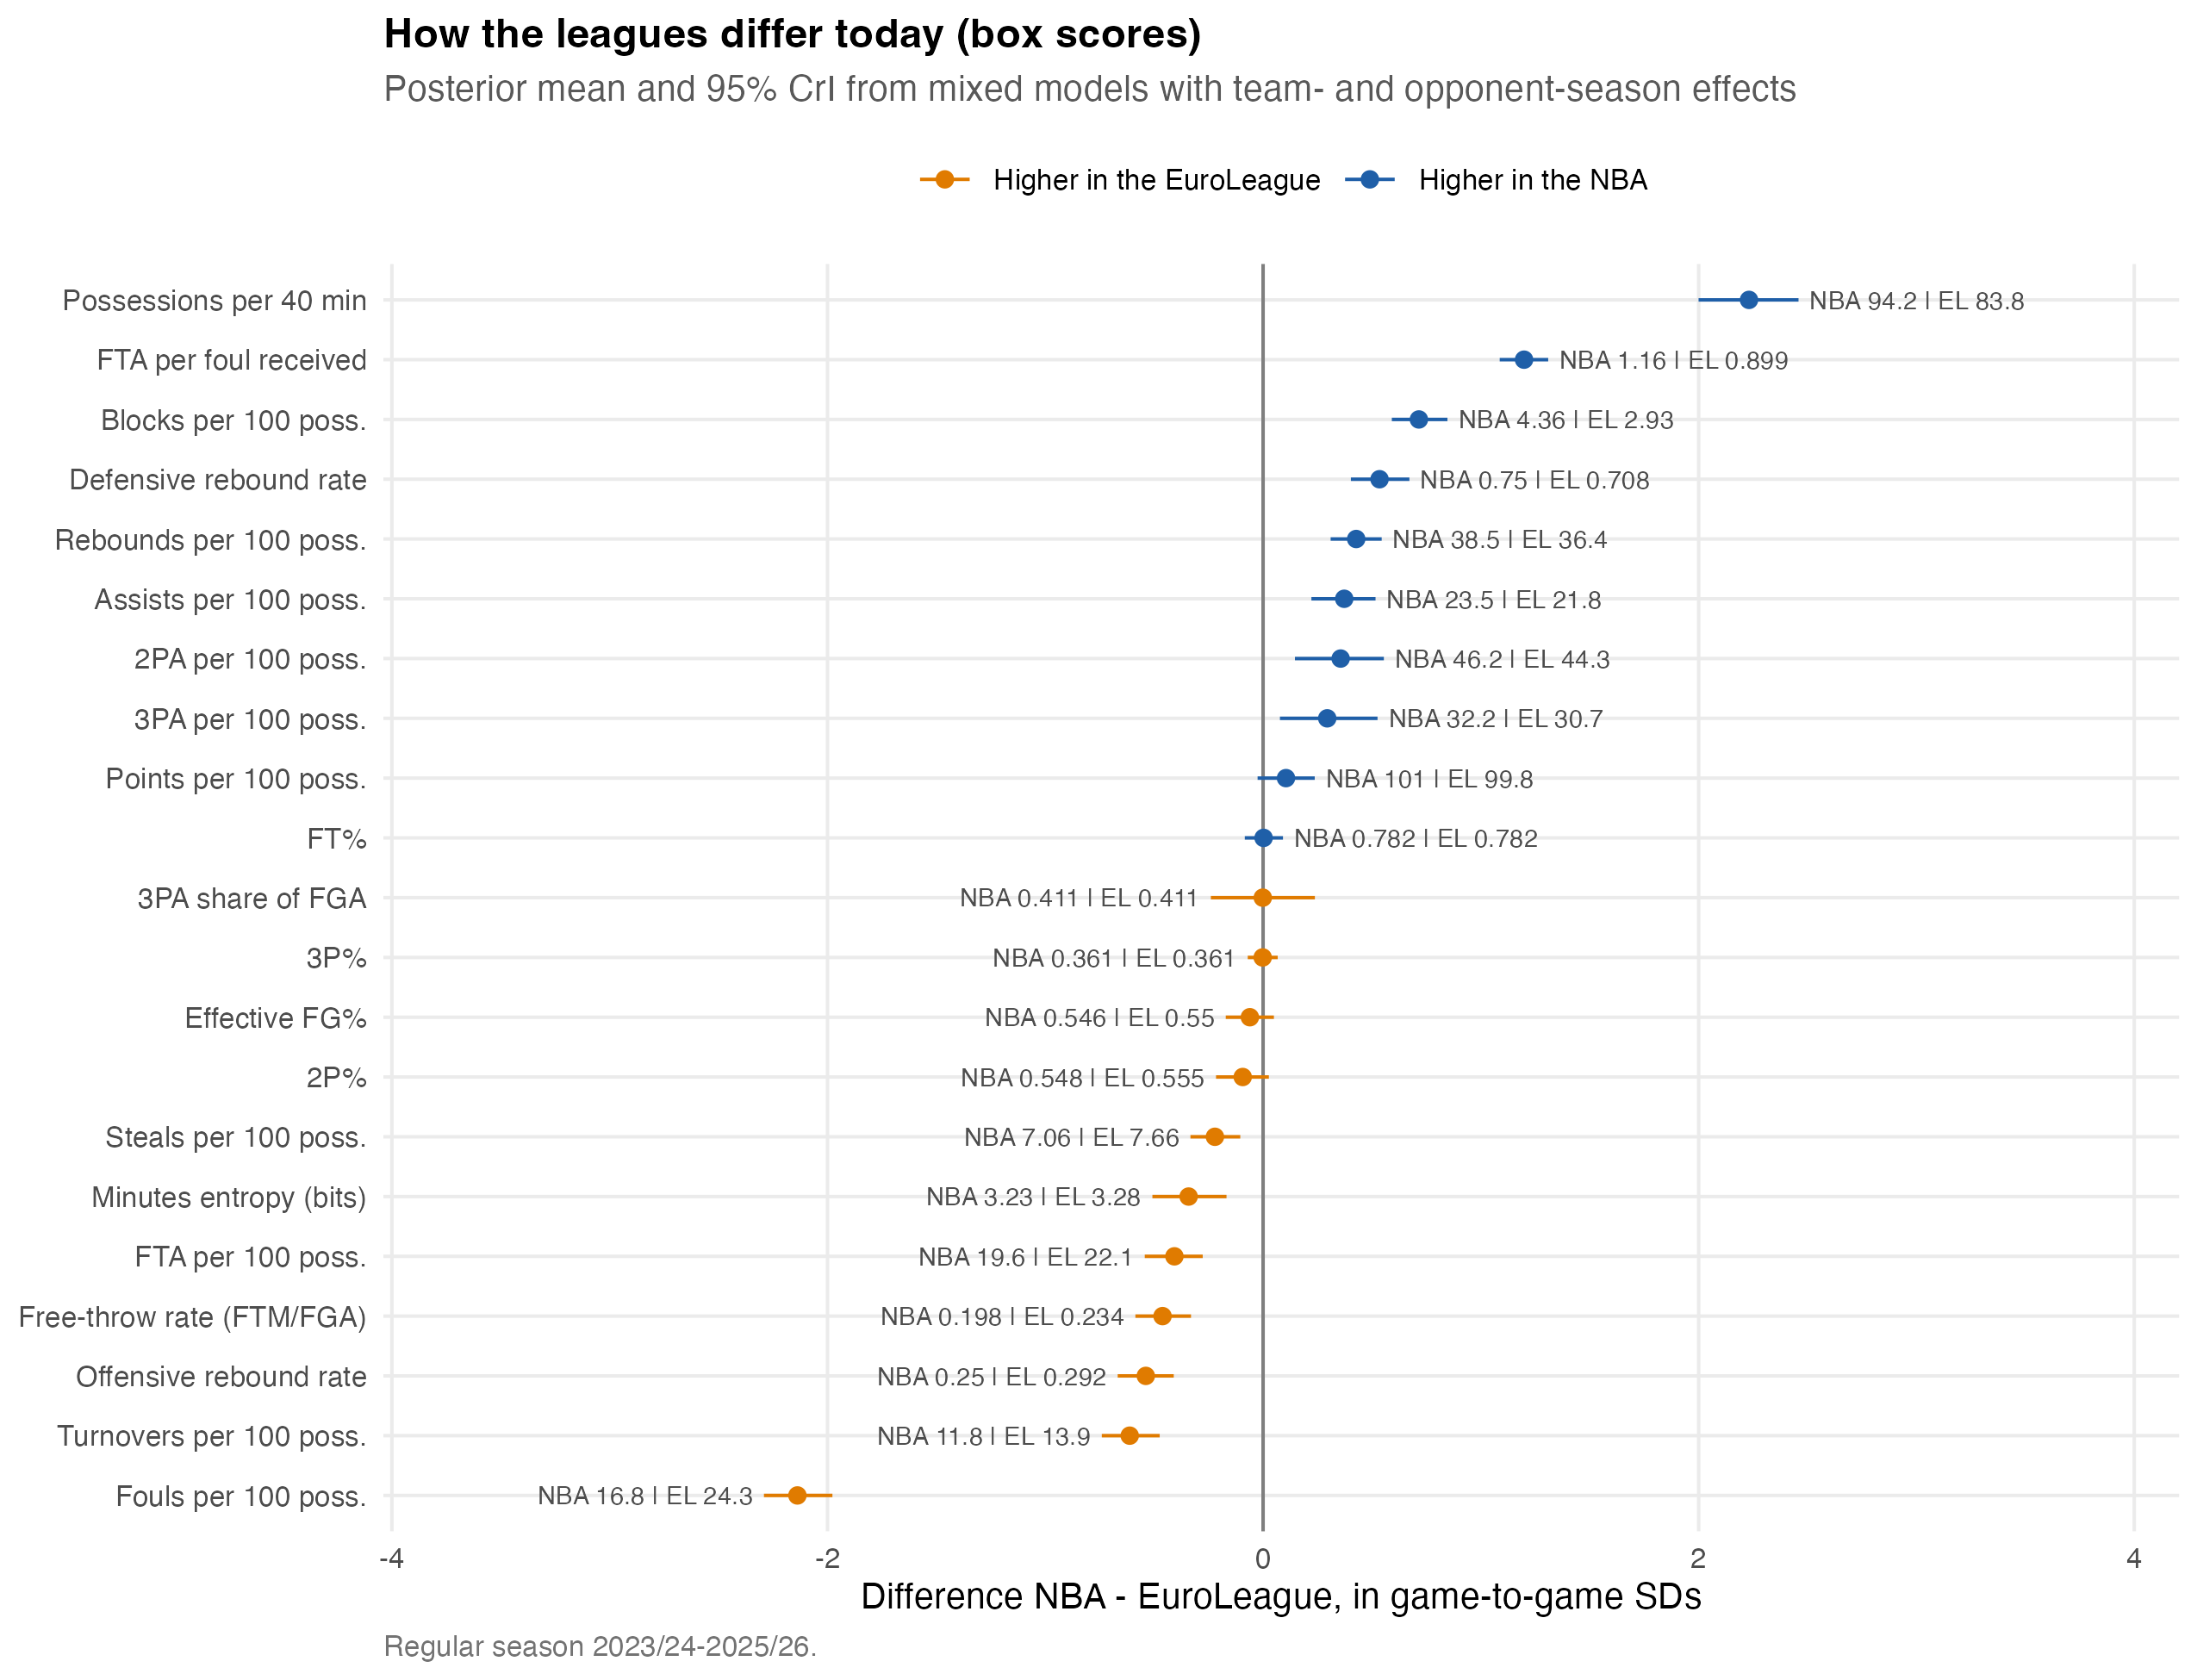
\includegraphics[width=0.92\textwidth,height=\textheight]{../RQ1_differences_today/results/figures/fig5_box_differences.png}

}

\caption{\label{fig-box}Box-score differences between the leagues,
regular season 2023/24--2025/26. Posterior means and 95\% credible
intervals from mixed models with team- and opponent-season effects, in
game-to-game standard deviations; numbers are the leagues' values on the
original scale.}

\end{figure}%

The equal three-point share hides different shot locations
(Figure~\ref{fig-shots}, Figure~\ref{fig-zones}). 11\% of NBA shots come
from the corner against 4\% in the EuroLeague, which instead takes more
above-the-break threes (36\% against 30\%) and more short mid-range
shots (21\% against 16\%). The rare EuroLeague corner three is worth
more: 1.28 points per shot against 1.16 in the NBA. In both leagues
threes are taken from just behind the league's own line, and beyond 2.5
m accuracy is the same; EuroLeague accuracy falls off faster on the
mid-range wings and far beyond the arc (Figure~\ref{fig-surface}).

\begin{figure}[htbp]

\centering{

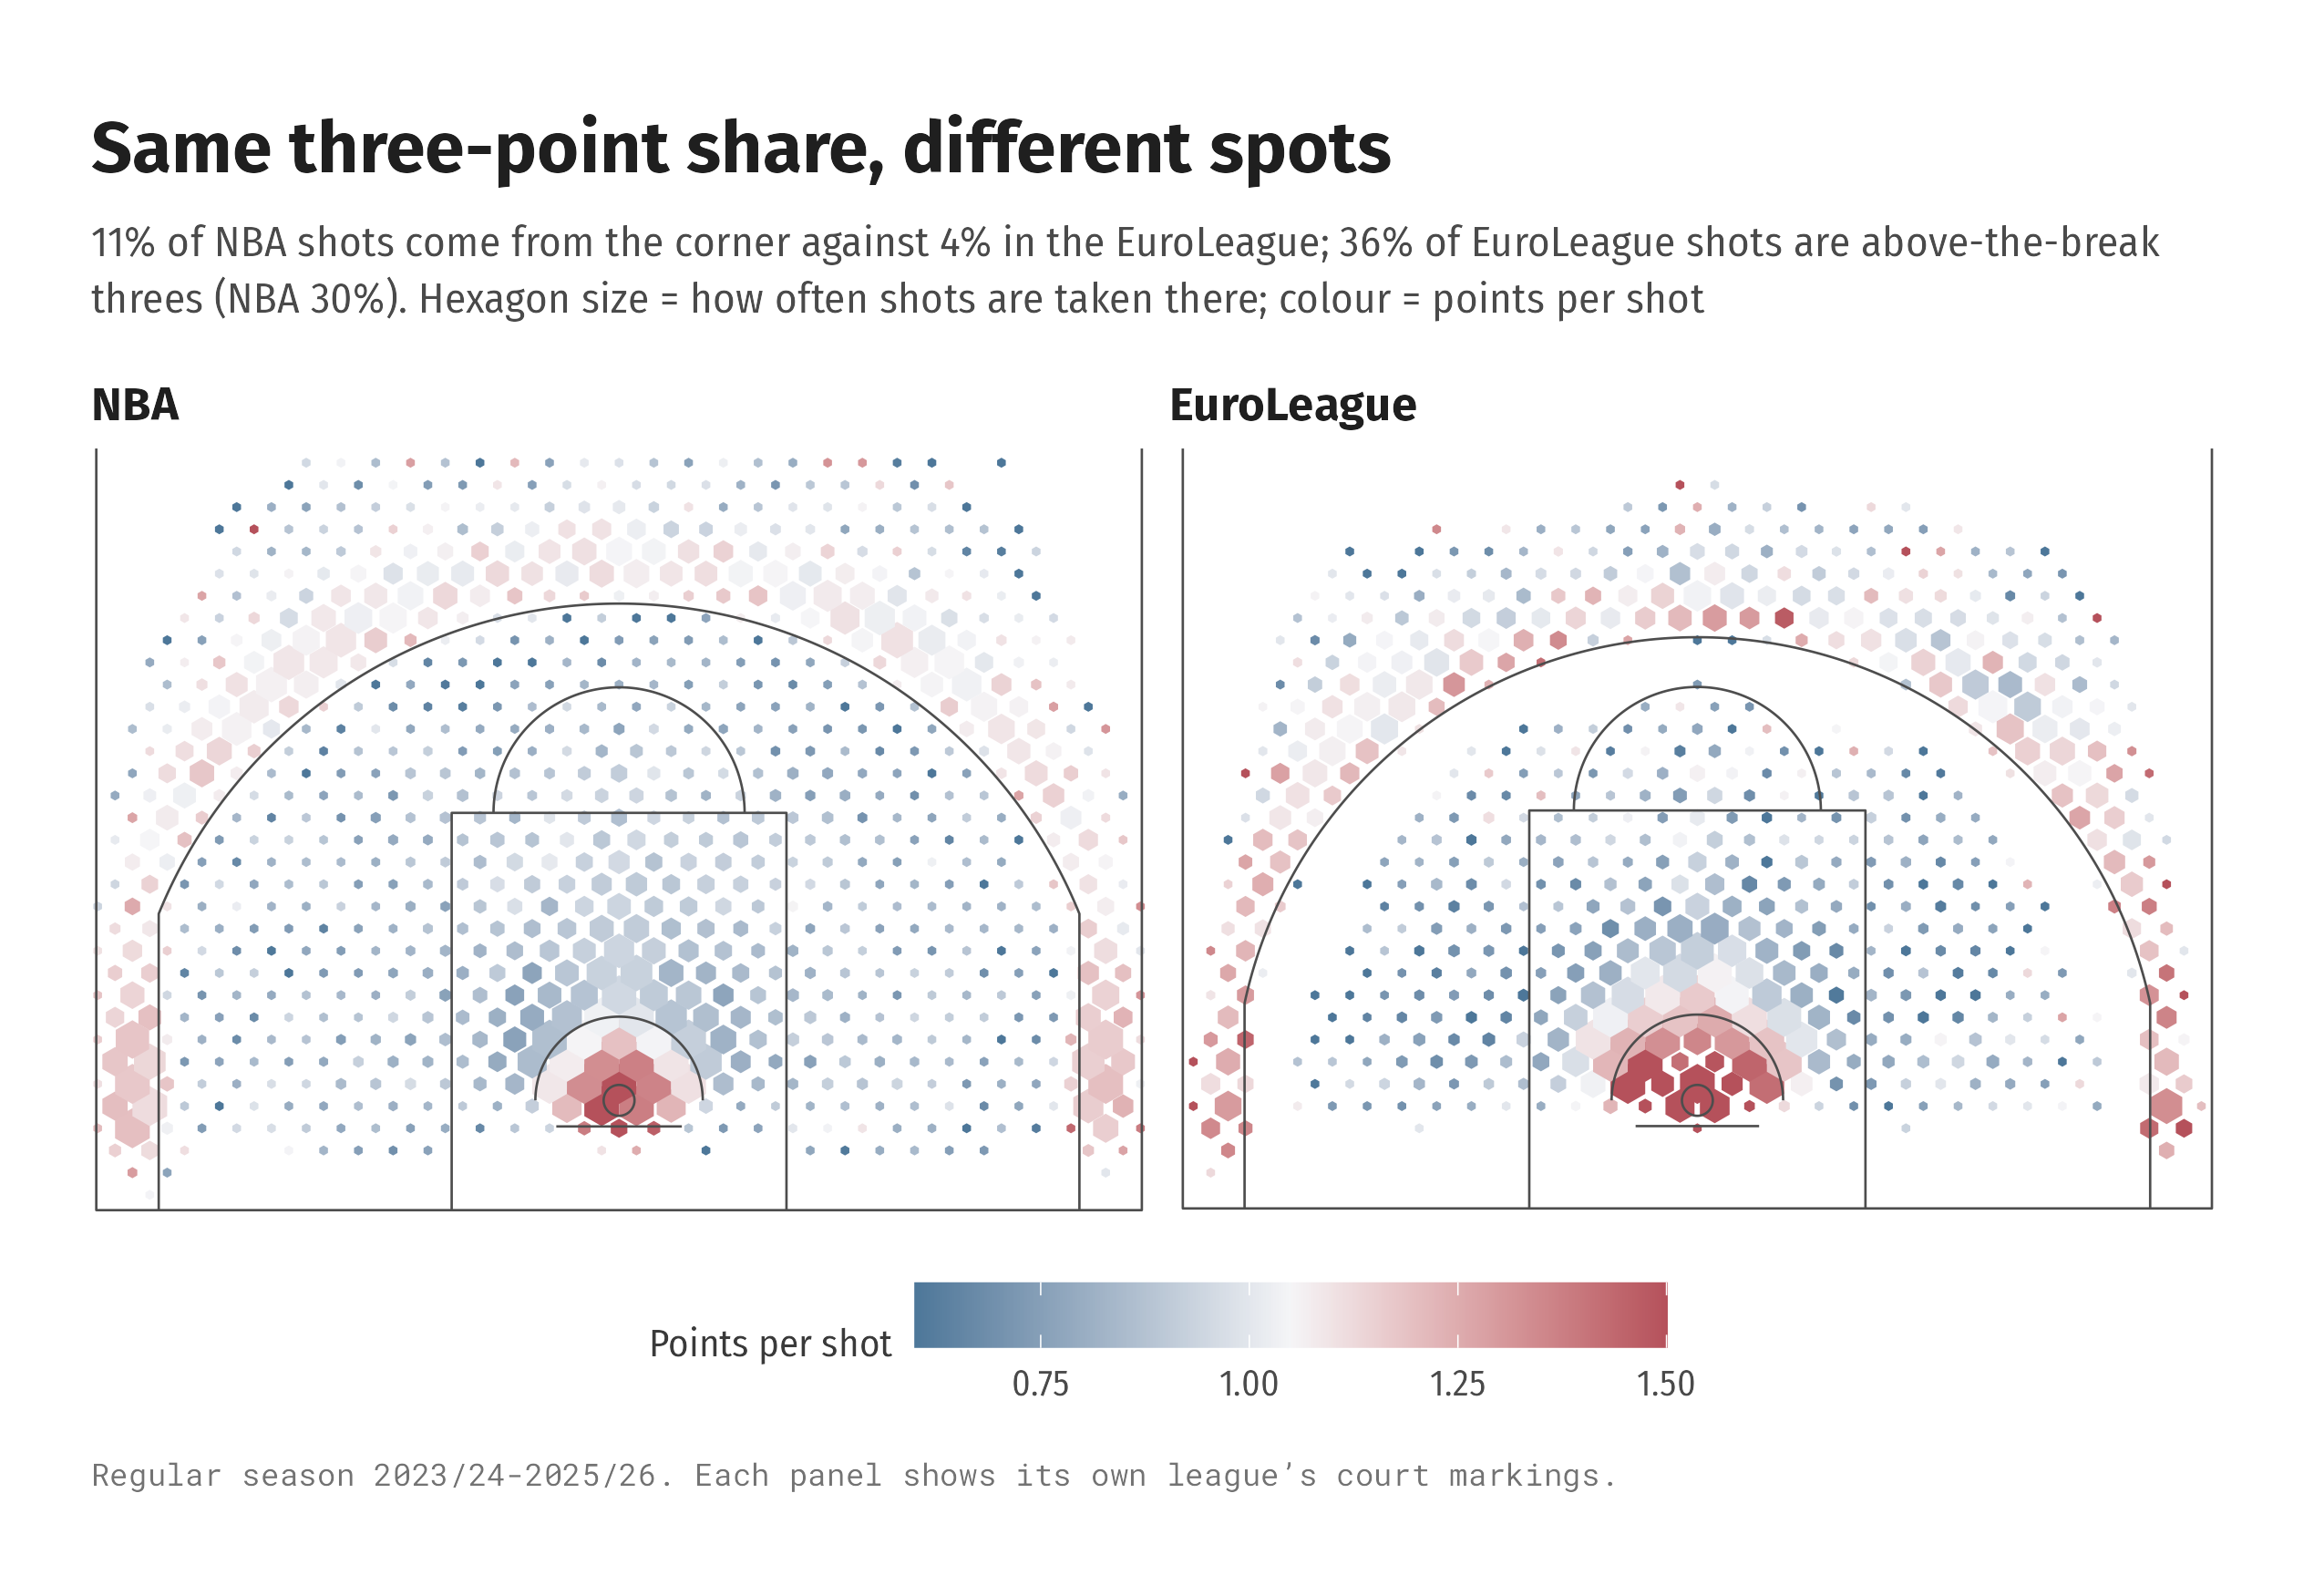
\includegraphics[width=0.92\textwidth,height=\textheight]{../RQ1_differences_today/results/figures/fig1_shot_charts_today.png}

}

\caption{\label{fig-shots}Shot charts, regular season 2023/24--2025/26.
Hexagon size = how often shots are taken from there; colour = points per
shot.}

\end{figure}%

\begin{figure}[htbp]

\centering{

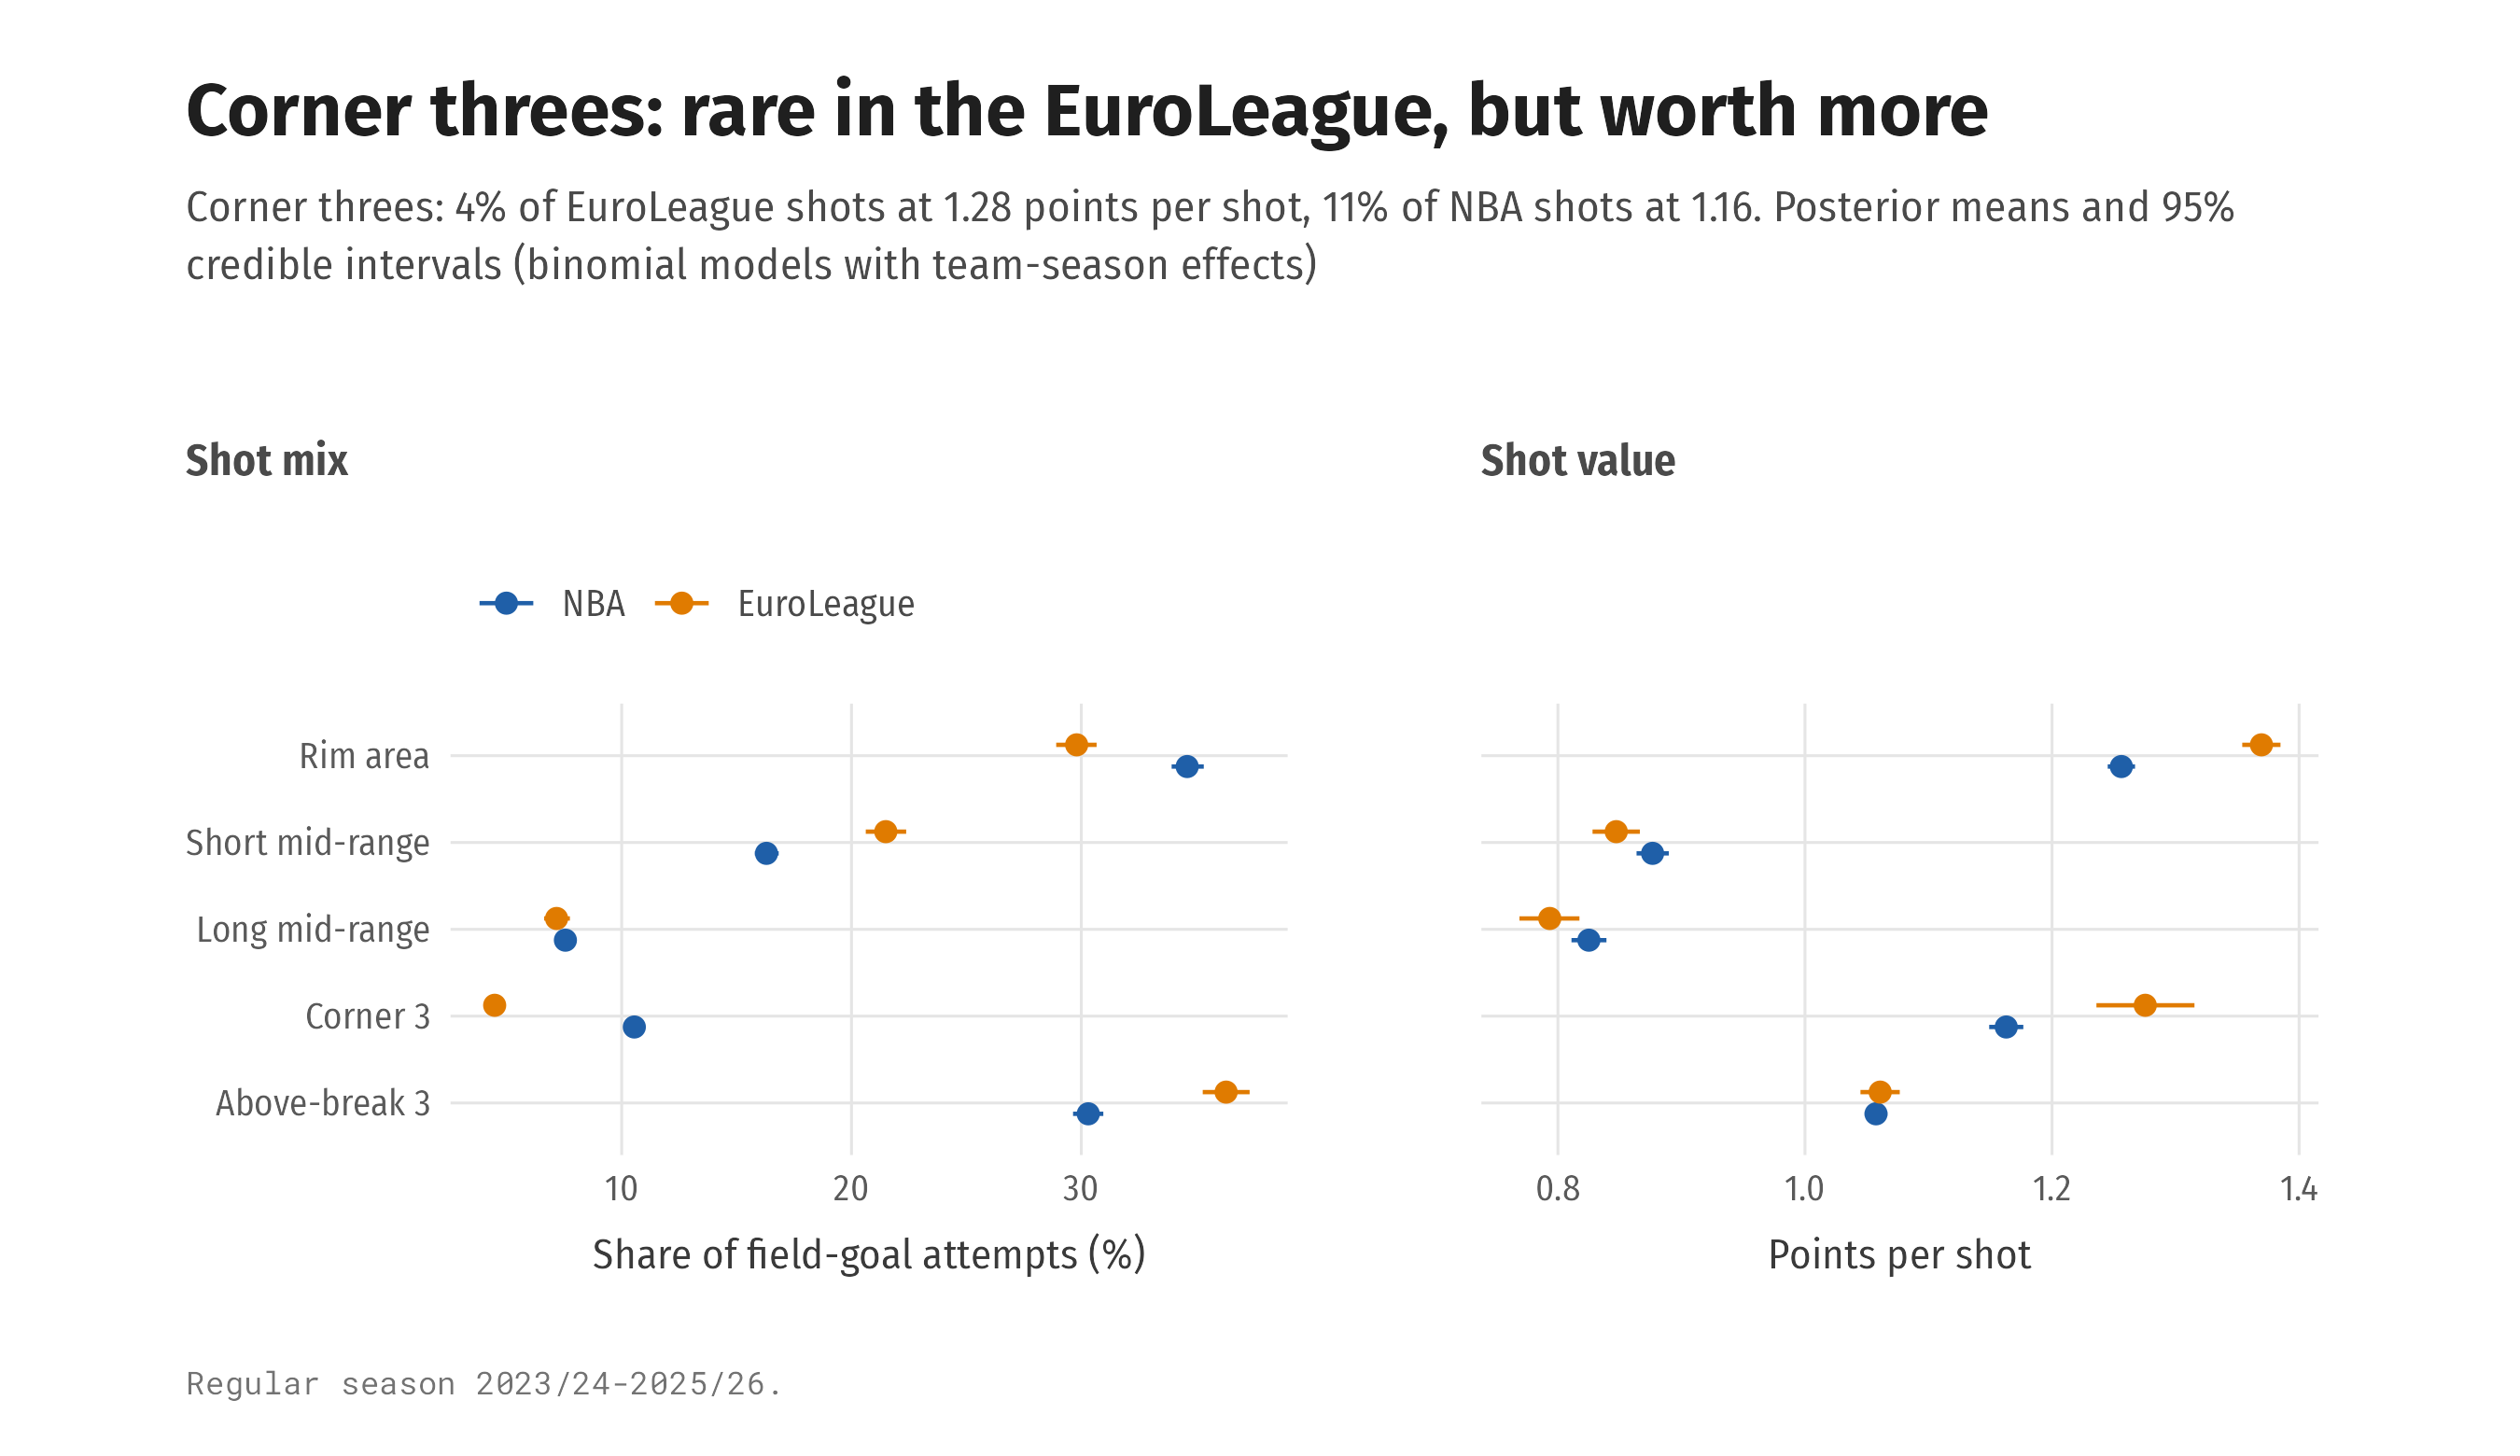
\includegraphics[width=0.92\textwidth,height=\textheight]{../RQ1_differences_today/results/figures/fig3_zone_profile.png}

}

\caption{\label{fig-zones}Shot share and value by zone for a typical
team. Posterior means and 95\% credible intervals from binomial models
with team-season effects.}

\end{figure}%

\begin{figure}[htbp]

\centering{

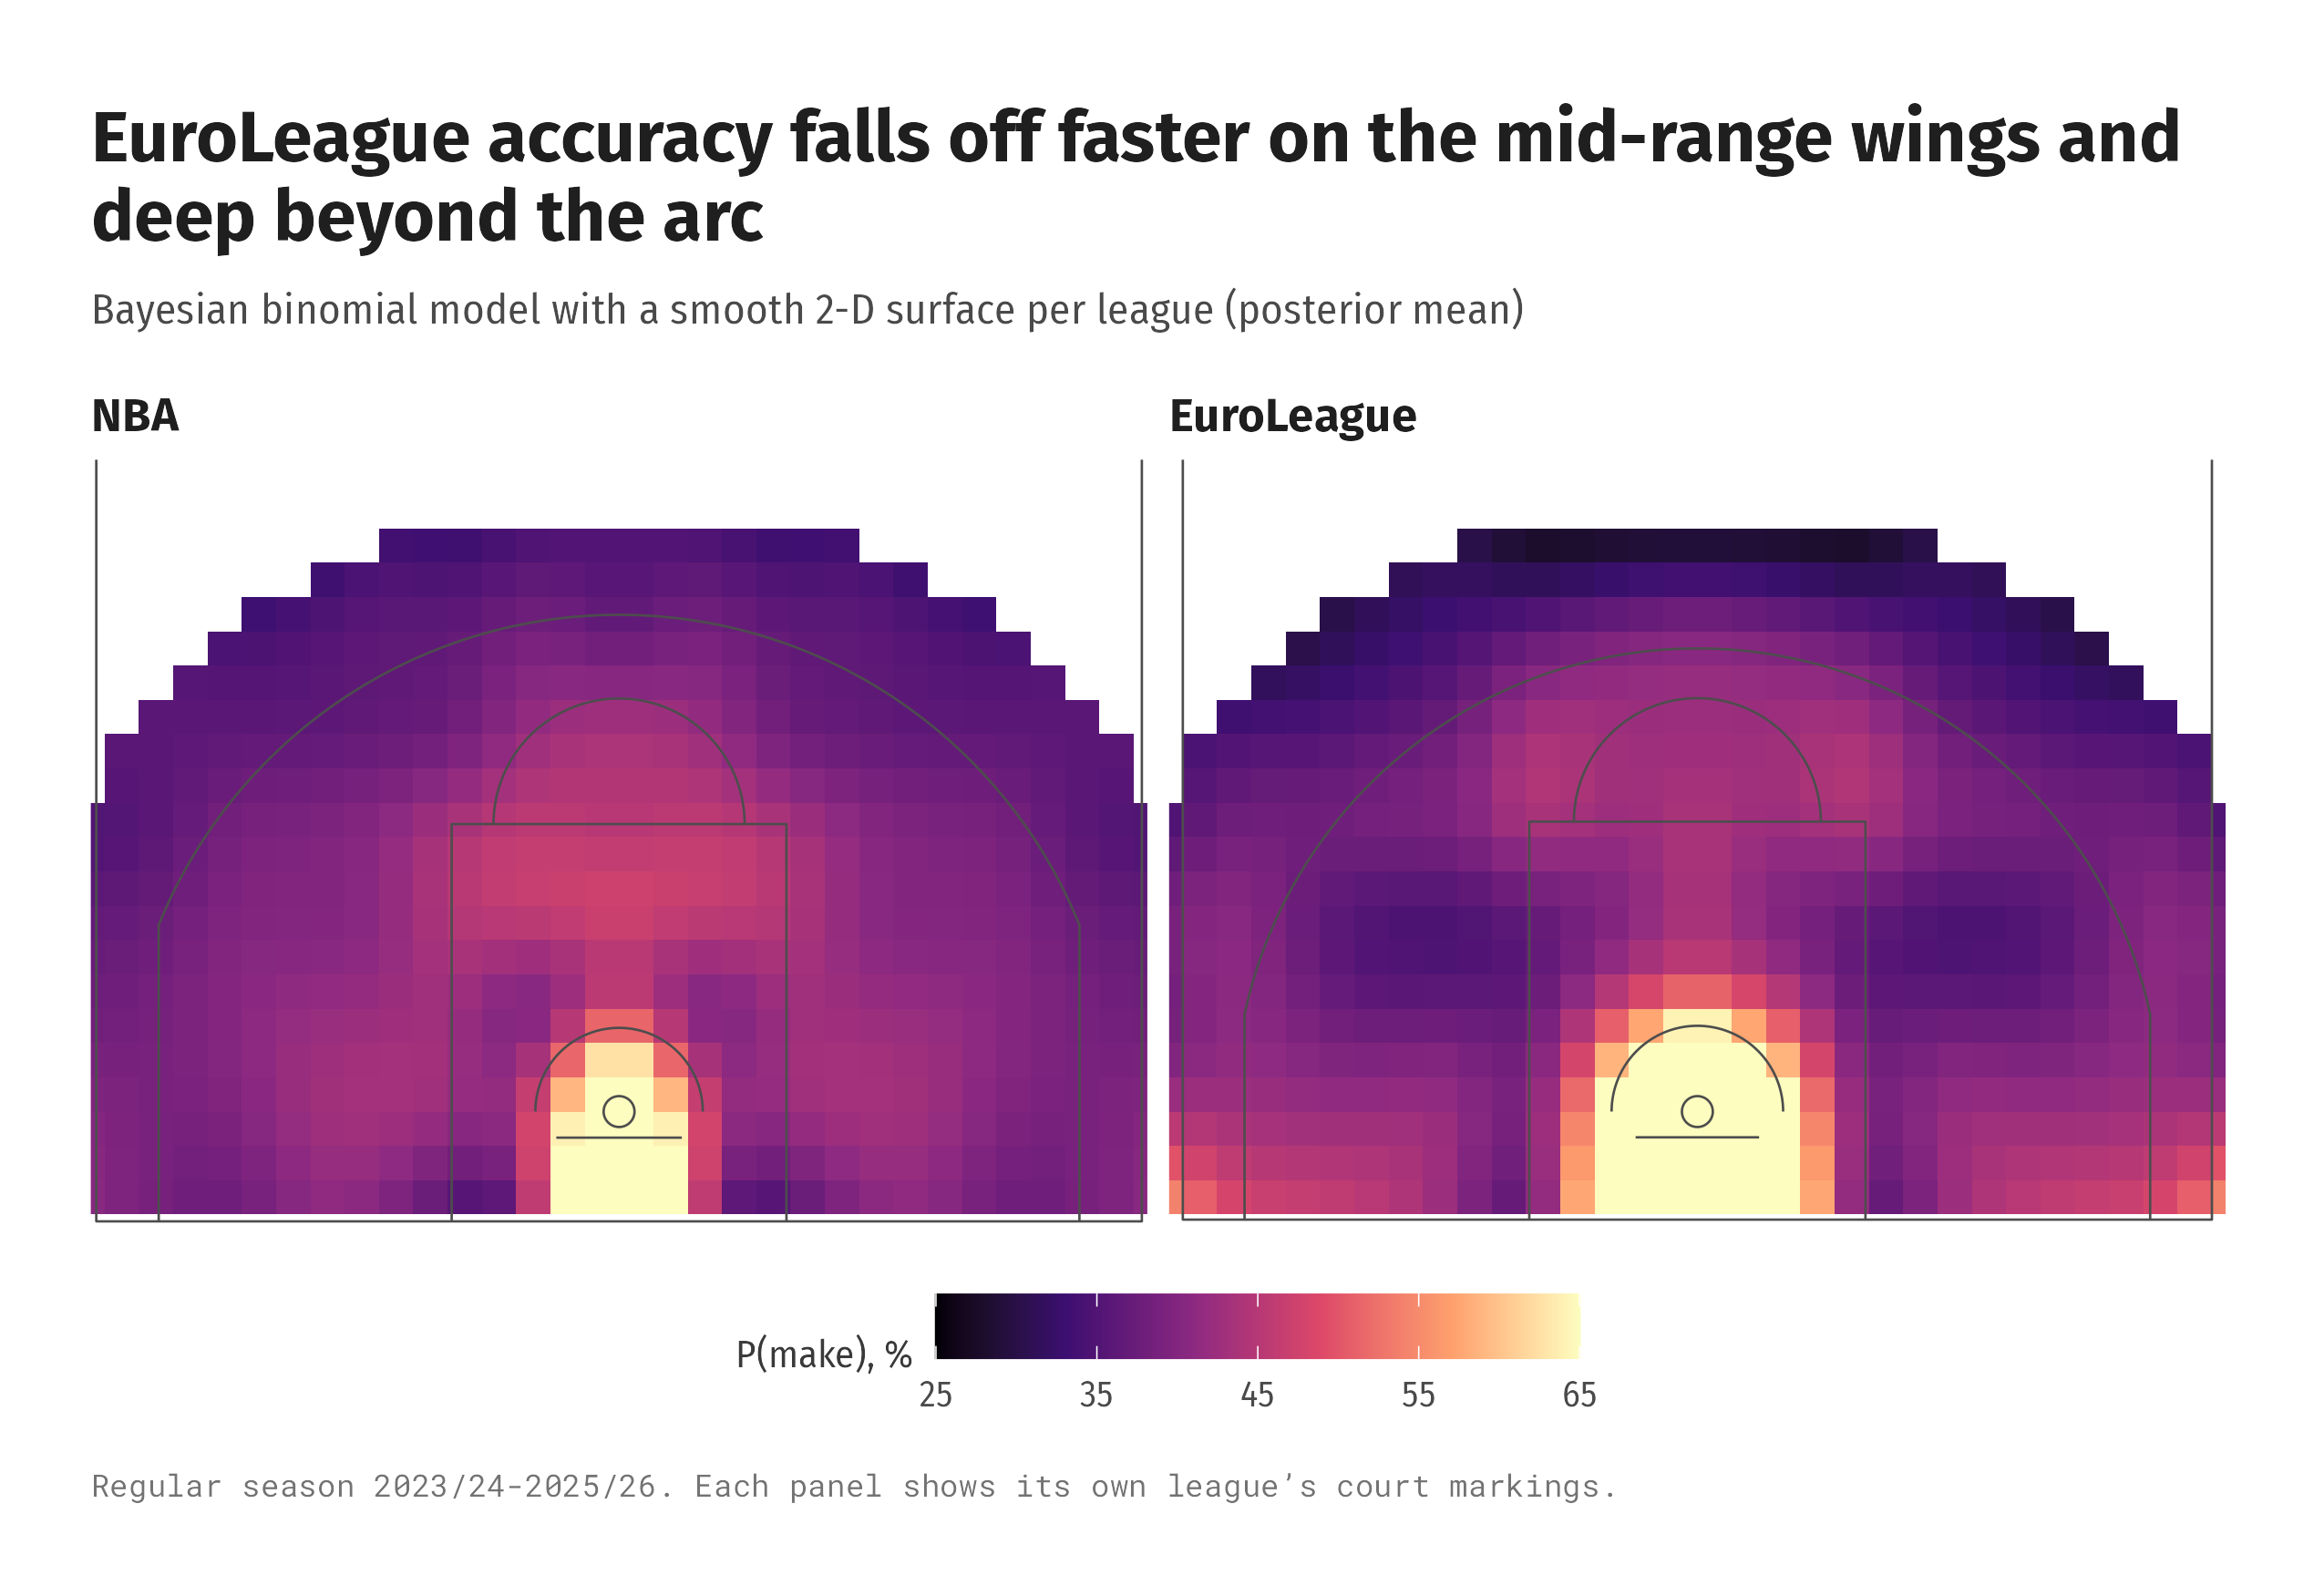
\includegraphics[width=0.92\textwidth,height=\textheight]{../RQ1_differences_today/results/figures/fig6_accuracy_surface.png}

}

\caption{\label{fig-surface}Modelled accuracy across the court: binomial
model with a smooth two-dimensional surface per league (posterior
mean).}

\end{figure}%

\subsection{How the leagues changed, and who follows whom
(RQ2)}\label{sec-replication}

\textbf{Replication.} Fitted to the 2019 paper's own data, our
implementation reproduces all 68 published estimates; the largest
absolute difference is 0.013 (Figure~\ref{fig-replication}).

\begin{figure}[htbp]

\centering{

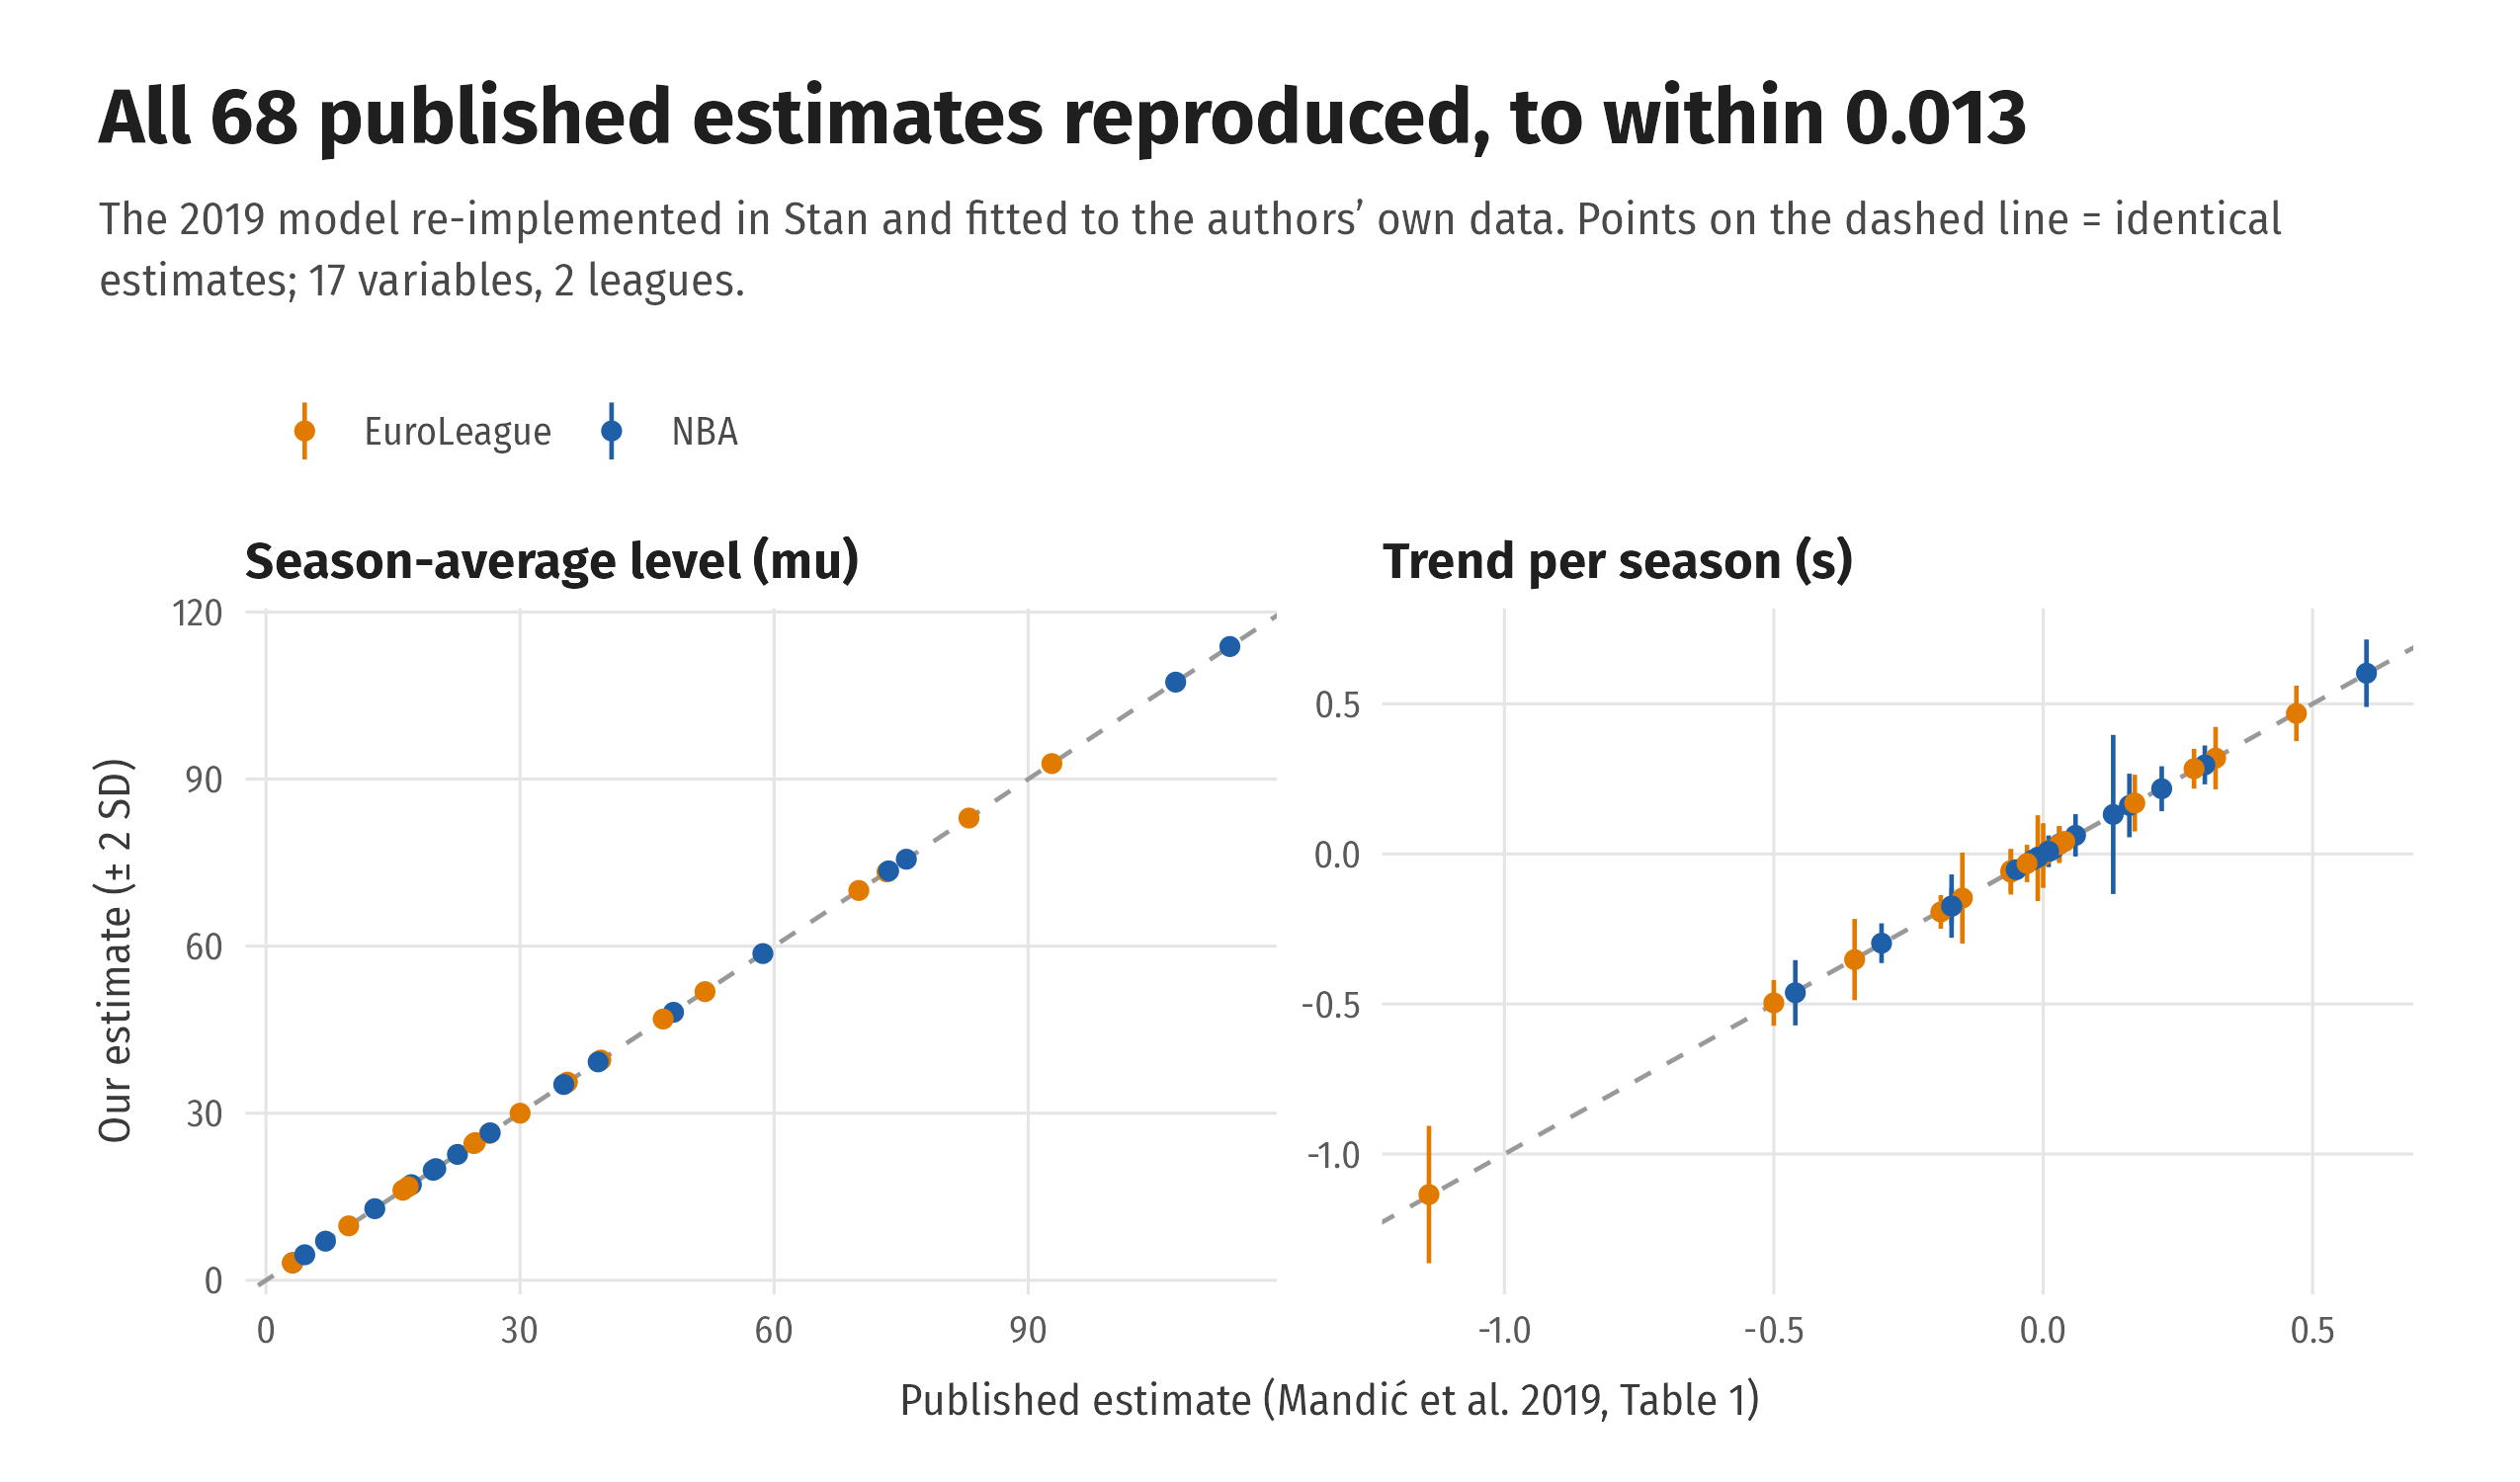
\includegraphics[width=0.75\textwidth,height=\textheight]{../RQ2_trends_leadlag/results/figures/rq2_replication_check.png}

}

\caption{\label{fig-replication}The 2019 model re-implemented in Stan
and fitted to the authors' published data, against their Table 1.}

\end{figure}%

\textbf{Trends.} Since 2010/11 both leagues have moved in the same
direction on most metrics (Figure~\ref{fig-trends}). The NBA closed an
11-point gap in three-point share: the gap went from -10.7 to 0.1
percentage points (probability that it shrank 1.00). Pace went the other
way: the gap grew from 6.7 to 9.6 possessions per 40 minutes
(probability that it shrank 0.003). Free-throw rate and offensive
rebounding also drifted apart (Figure~\ref{fig-convergence}).

\begin{figure}[htbp]

\centering{

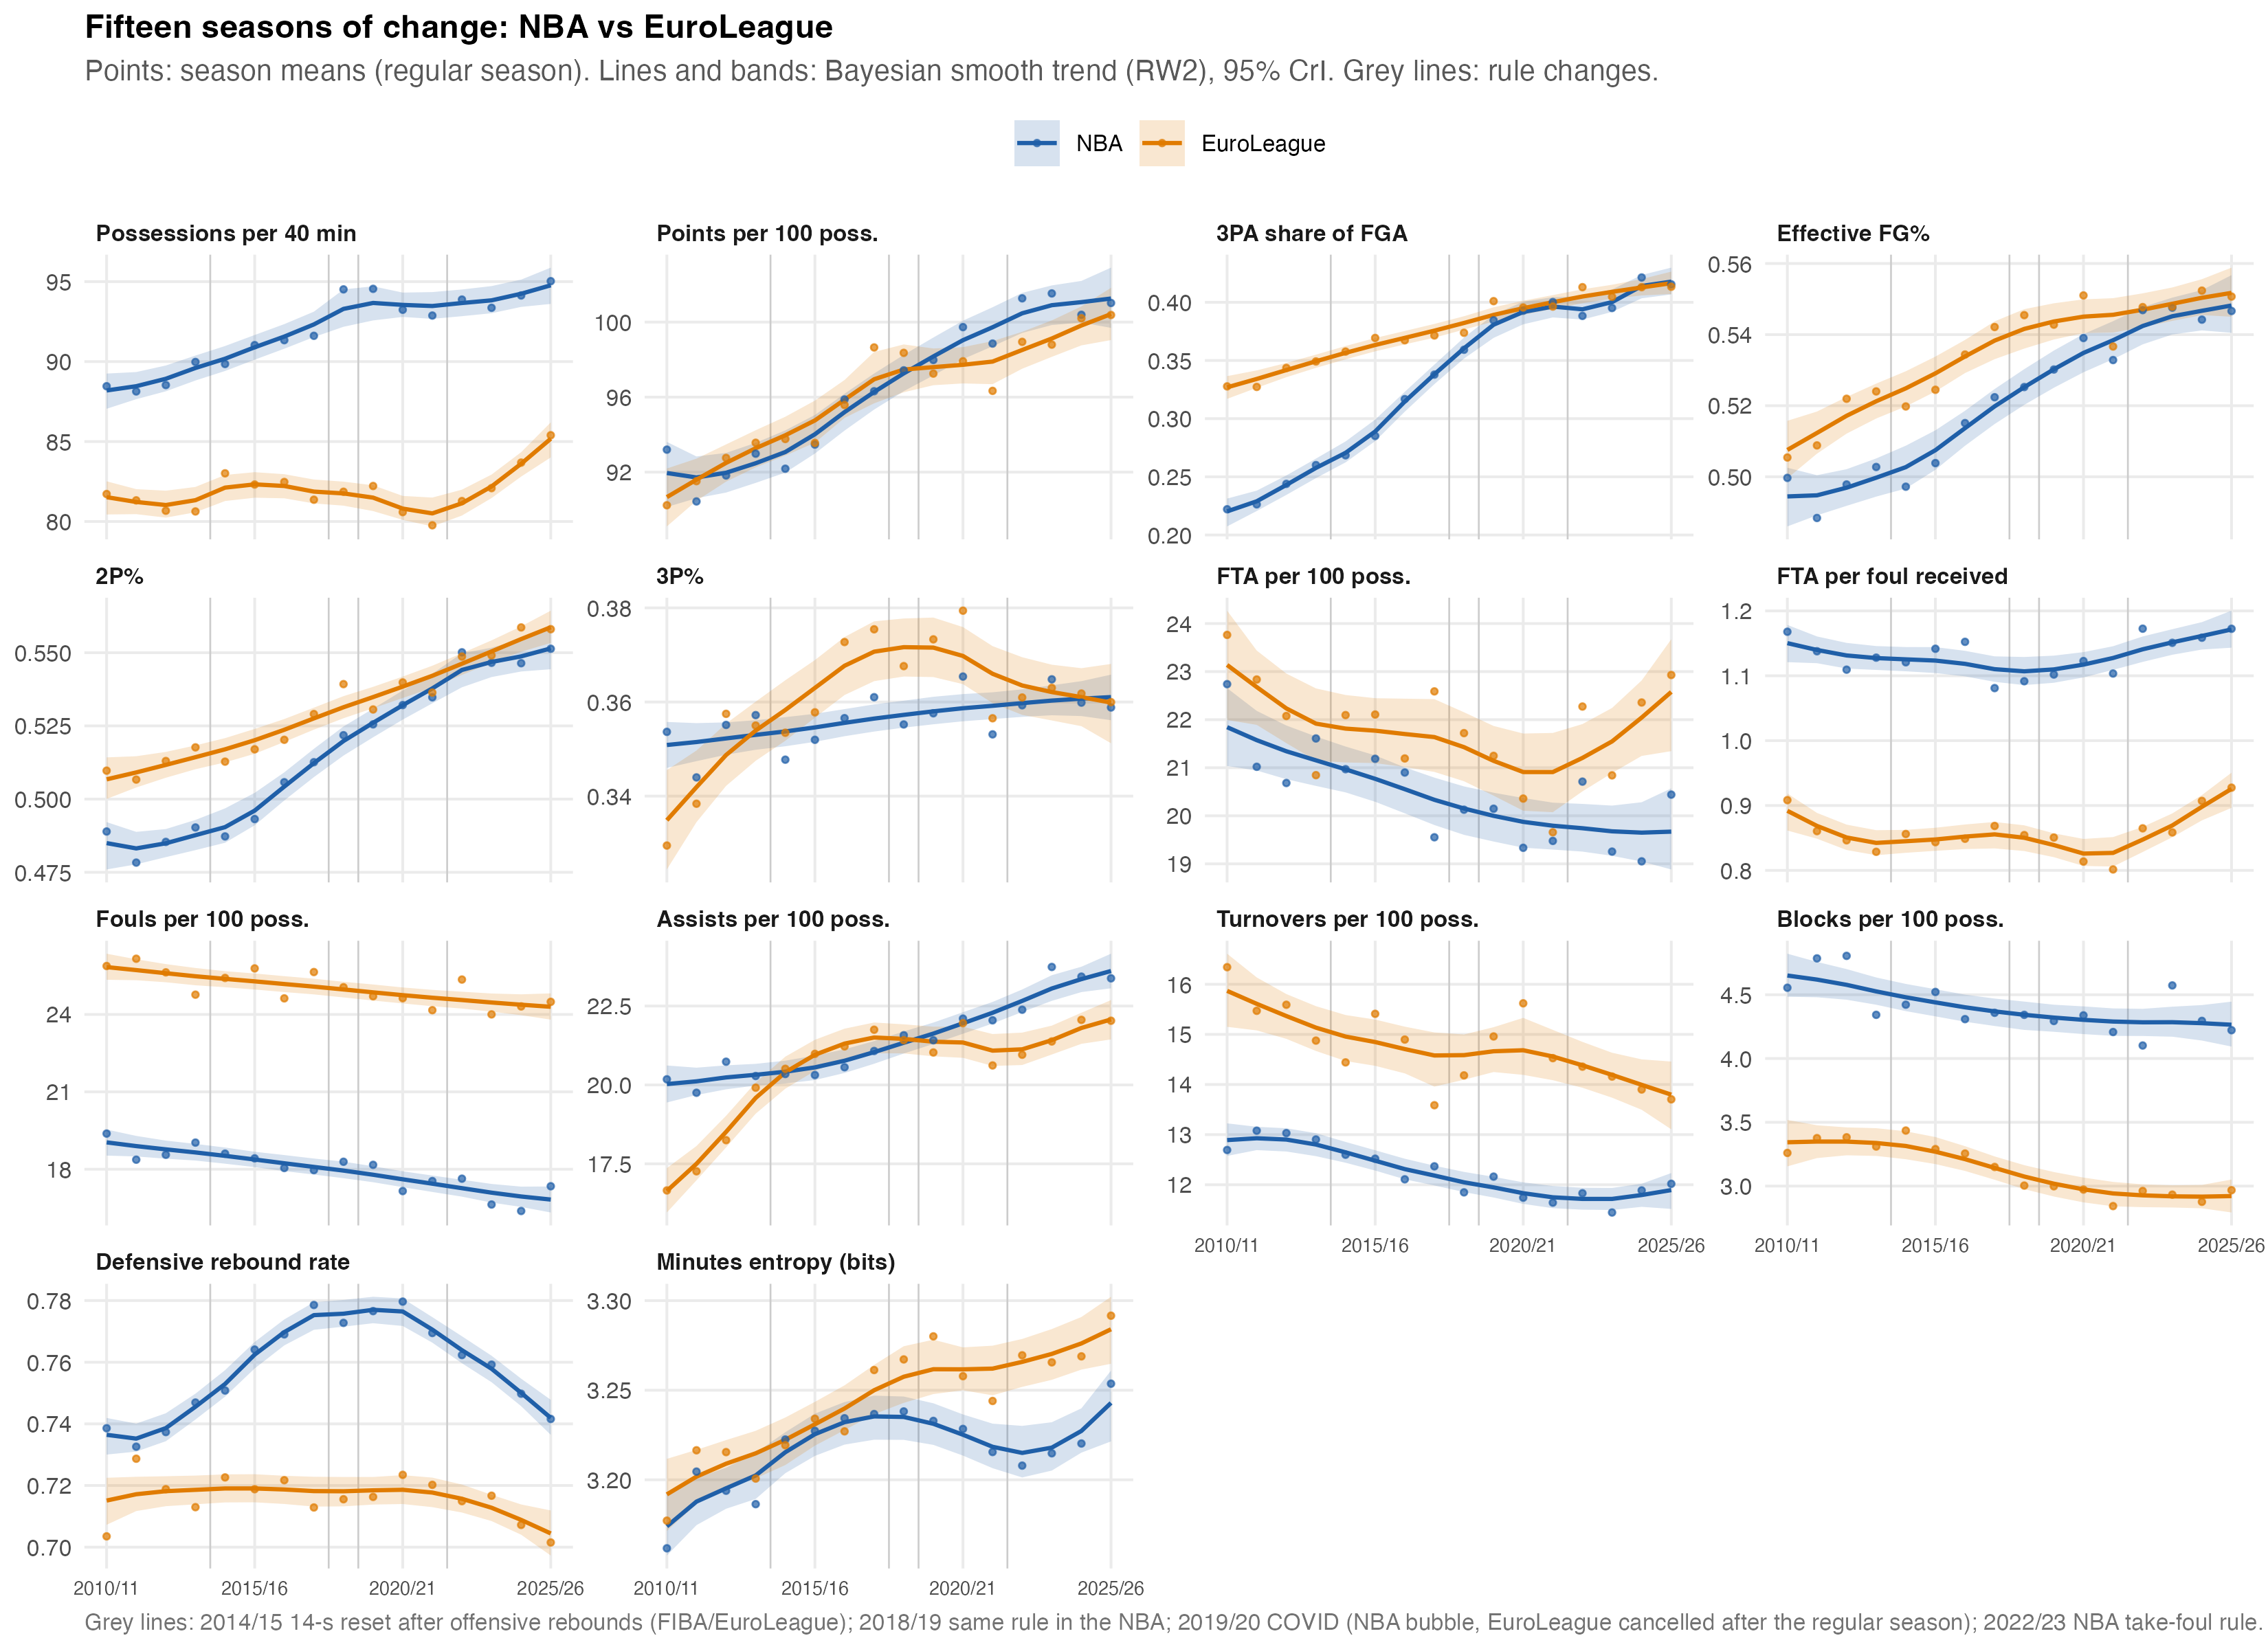
\includegraphics[width=11in,height=\textheight]{../RQ2_trends_leadlag/results/figures/fig1_trends.png}

}

\caption{\label{fig-trends}Season means (points) and Bayesian smooth
trends (RW2, 95\% credible bands), regular season 2010/11--2025/26. Grey
vertical lines mark rule changes.}

\end{figure}%

\begin{figure}[htbp]

\centering{

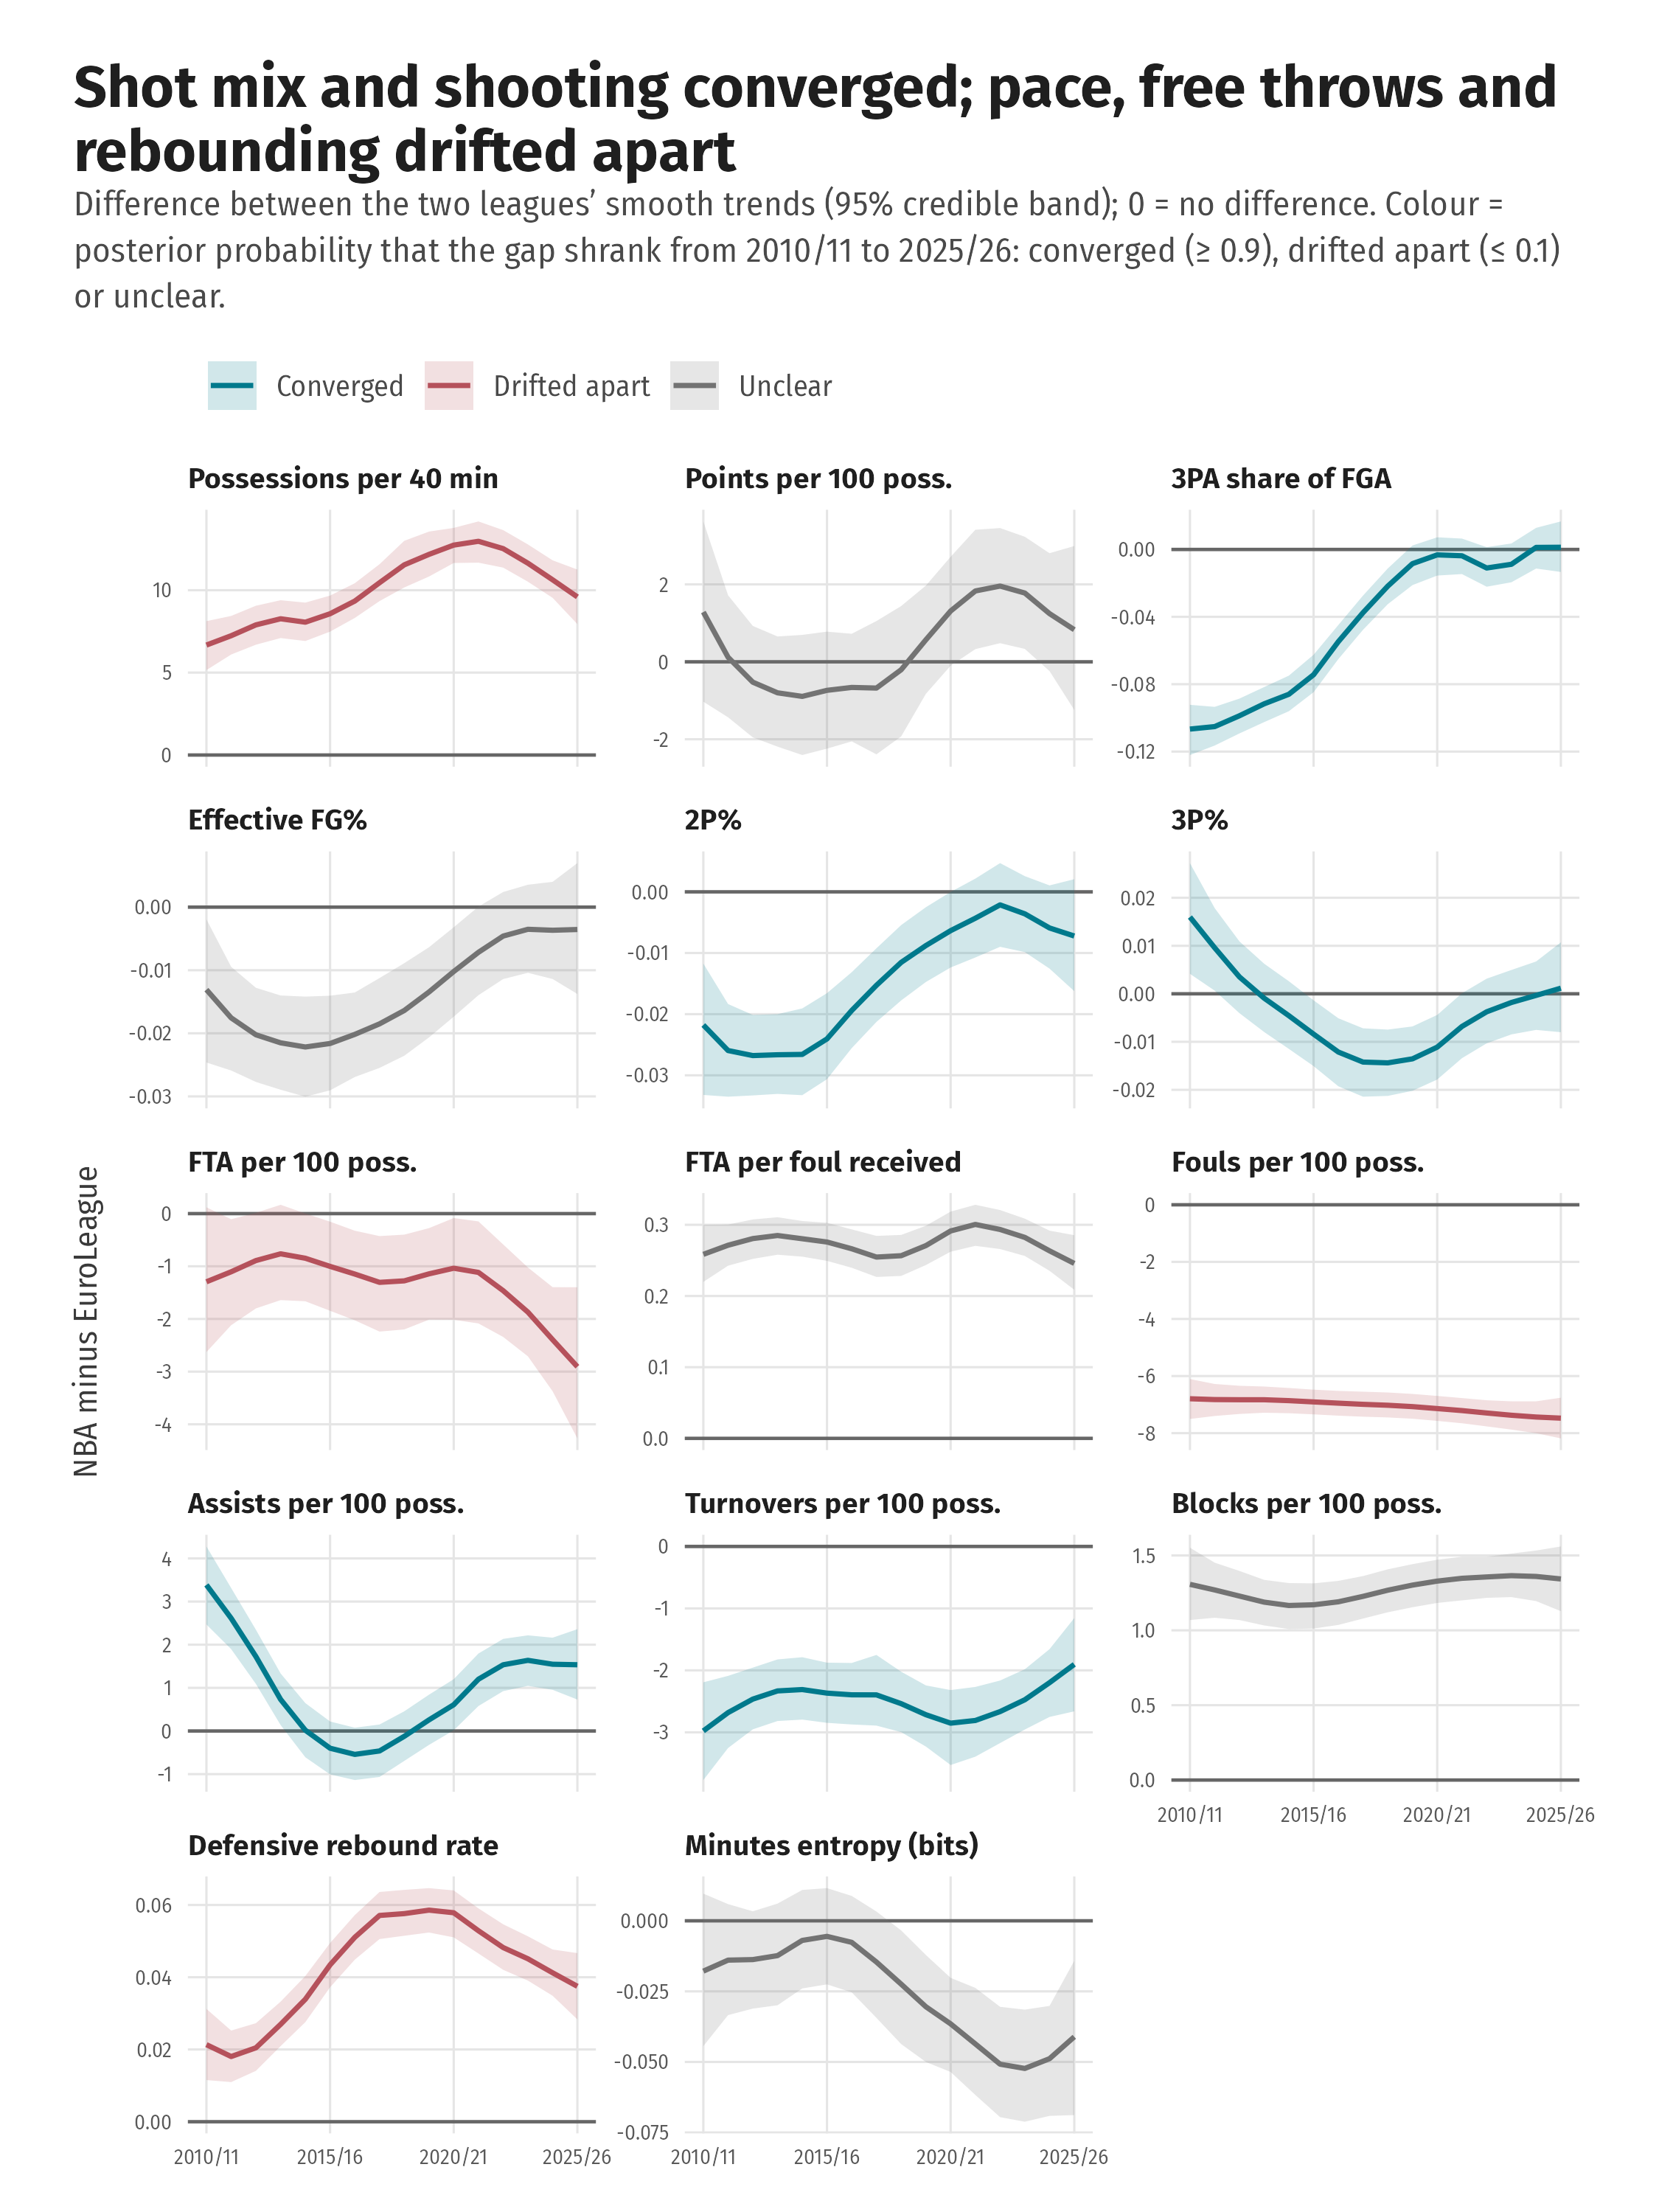
\includegraphics[width=11in,height=\textheight]{../RQ2_trends_leadlag/results/figures/fig2_convergence.png}

}

\caption{\label{fig-convergence}Gap between the leagues (NBA minus
EuroLeague) over time, 95\% credible bands. A line moving towards zero
means the leagues are converging.}

\end{figure}%

\textbf{Lead--lag.} For most metrics the shift model cannot say which
league leads (Figure~\ref{fig-leadlag}). The clearest signals concern
three-point shooting: on three-point attempts per 100 possessions the
leagues move in step (most probable lag 0, probability 0.50), and on the
share of shots from three the EuroLeague is in step or one season behind
(probability that it follows 0.65). On volume measures the EuroLeague of
2025/26 looks like the NBA of about 3 (points per 100 possessions), 4
(three-point attempts) and 5 (assists) seasons earlier
(Figure~\ref{fig-timegap}).

\begin{figure}[htbp]

\centering{

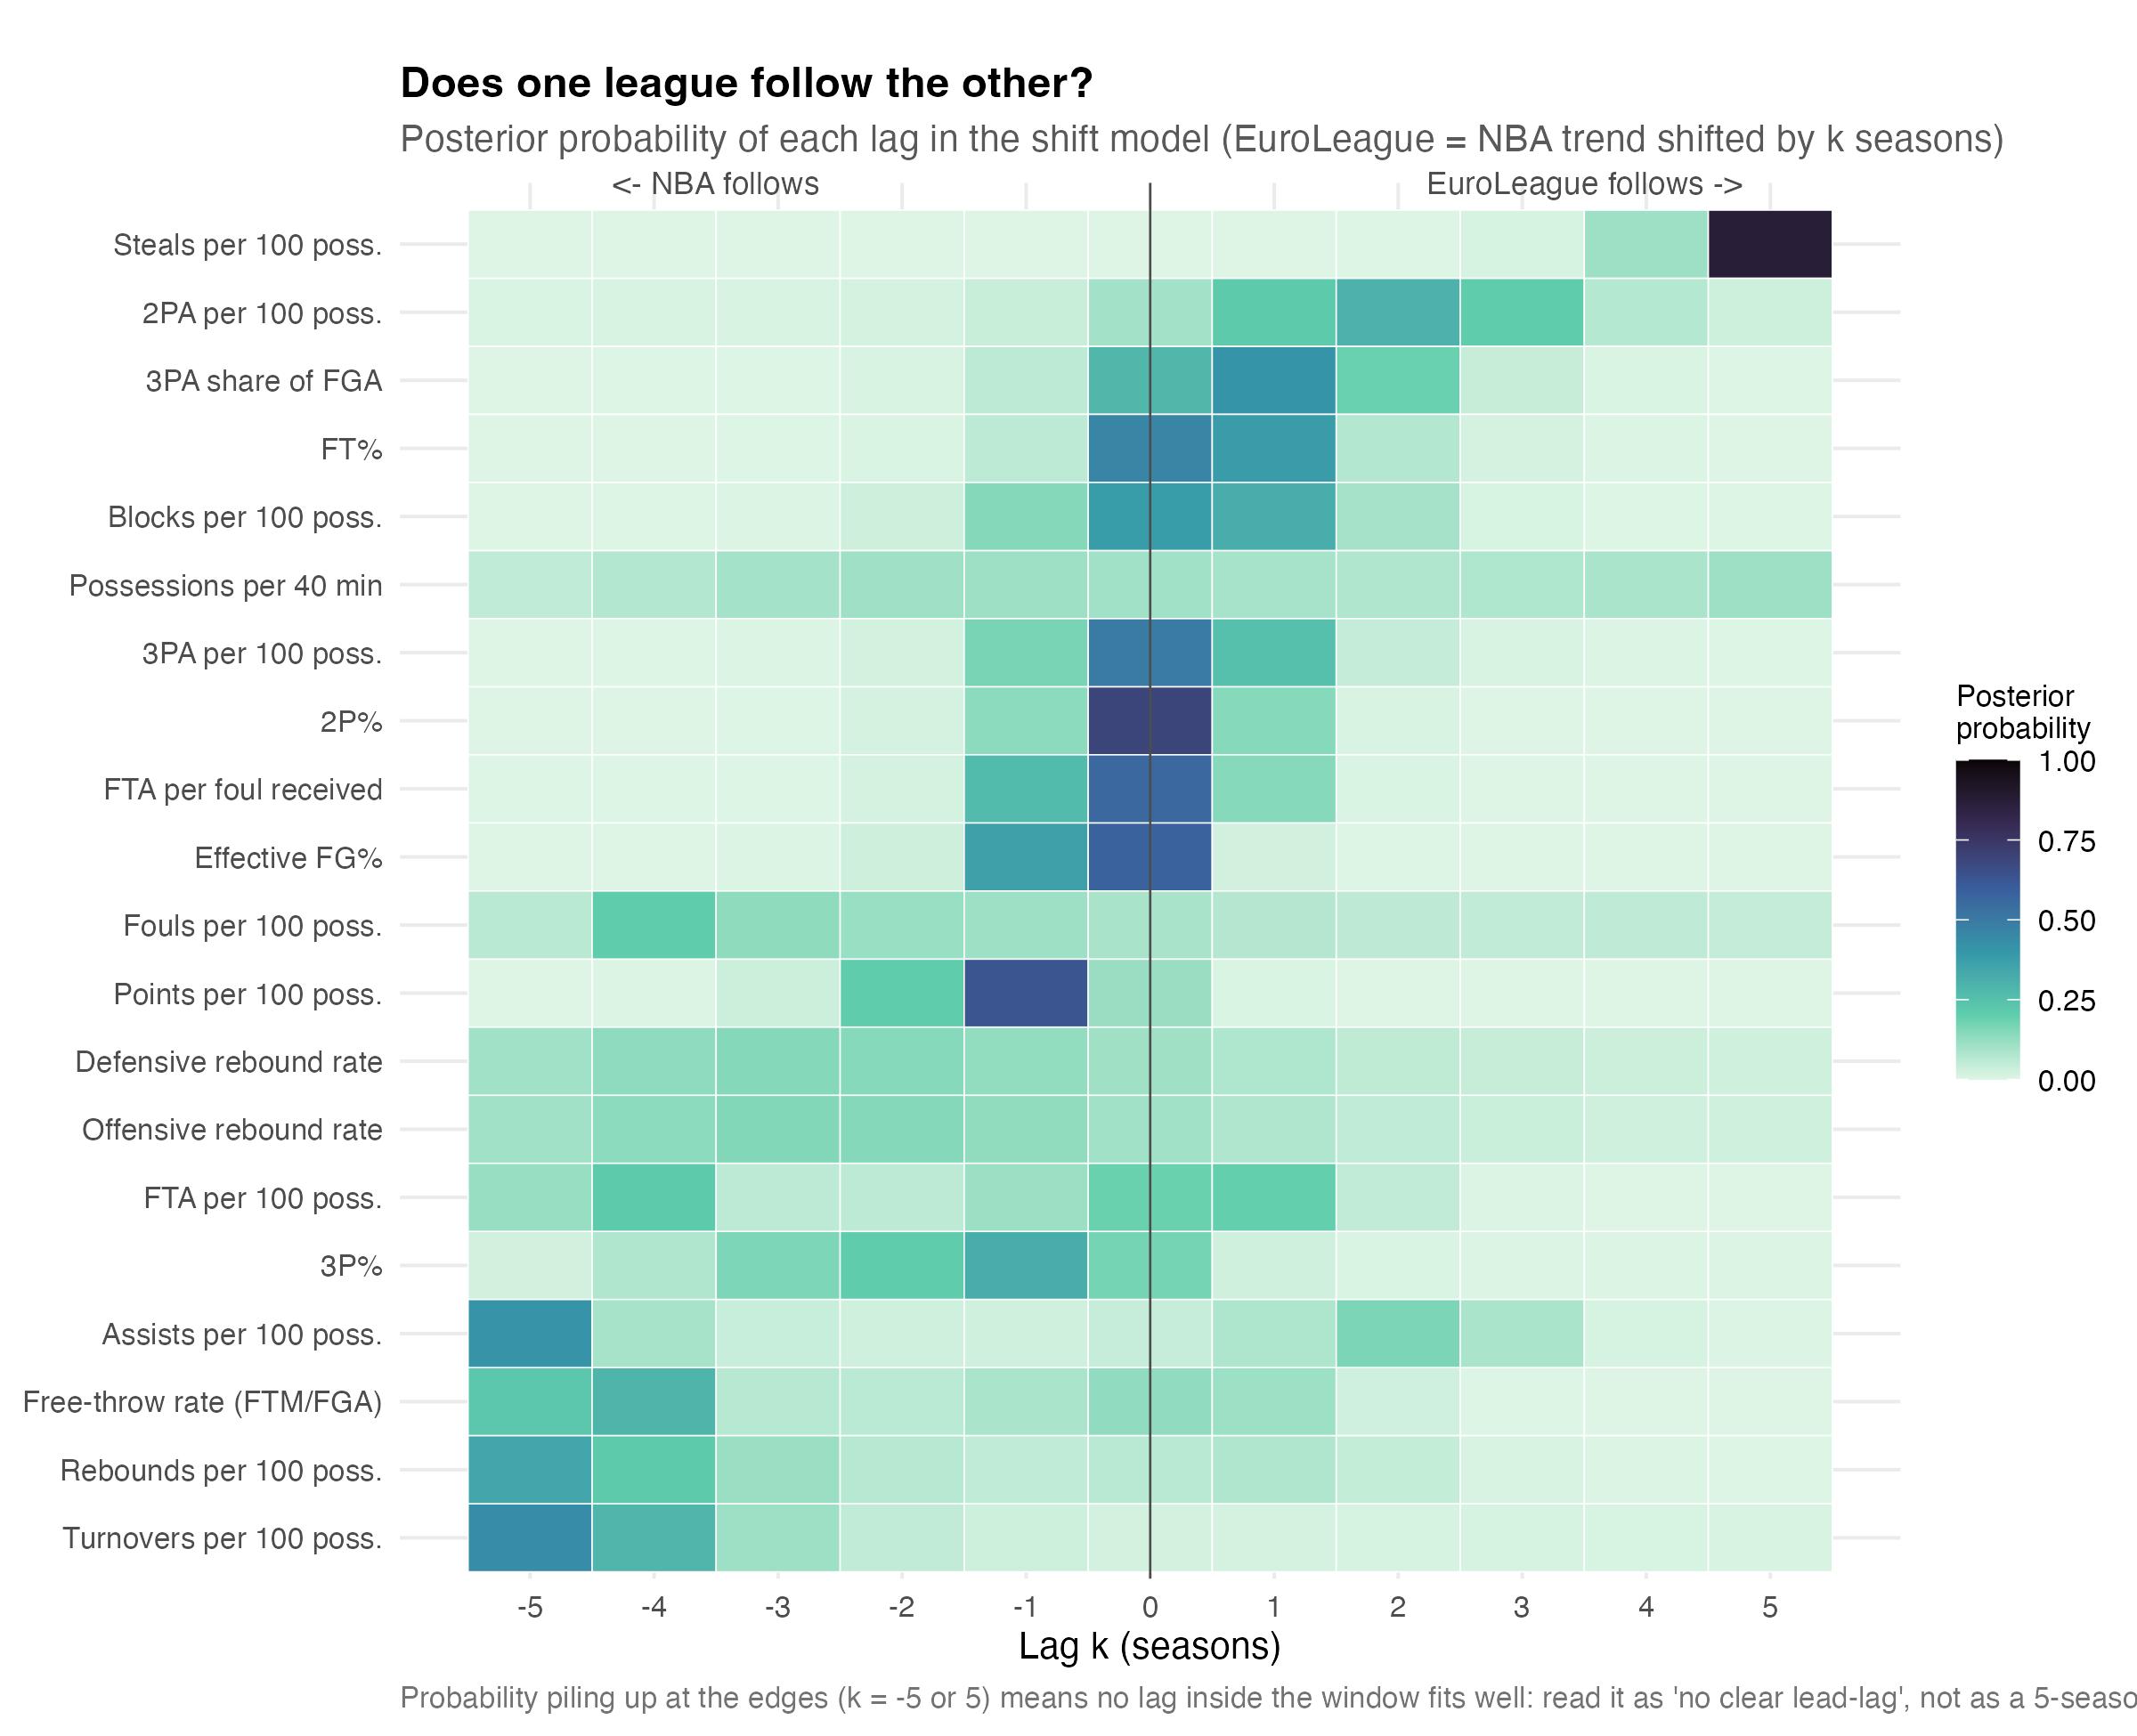
\includegraphics[width=0.85\textwidth,height=\textheight]{../RQ2_trends_leadlag/results/figures/fig3_lead_lag.png}

}

\caption{\label{fig-leadlag}Shift model: posterior probability that the
EuroLeague's trend equals the NBA's shifted by k seasons. Probability
piling up at k = ±5 means that no lag inside the window fits well.}

\end{figure}%

\begin{figure}[htbp]

\centering{

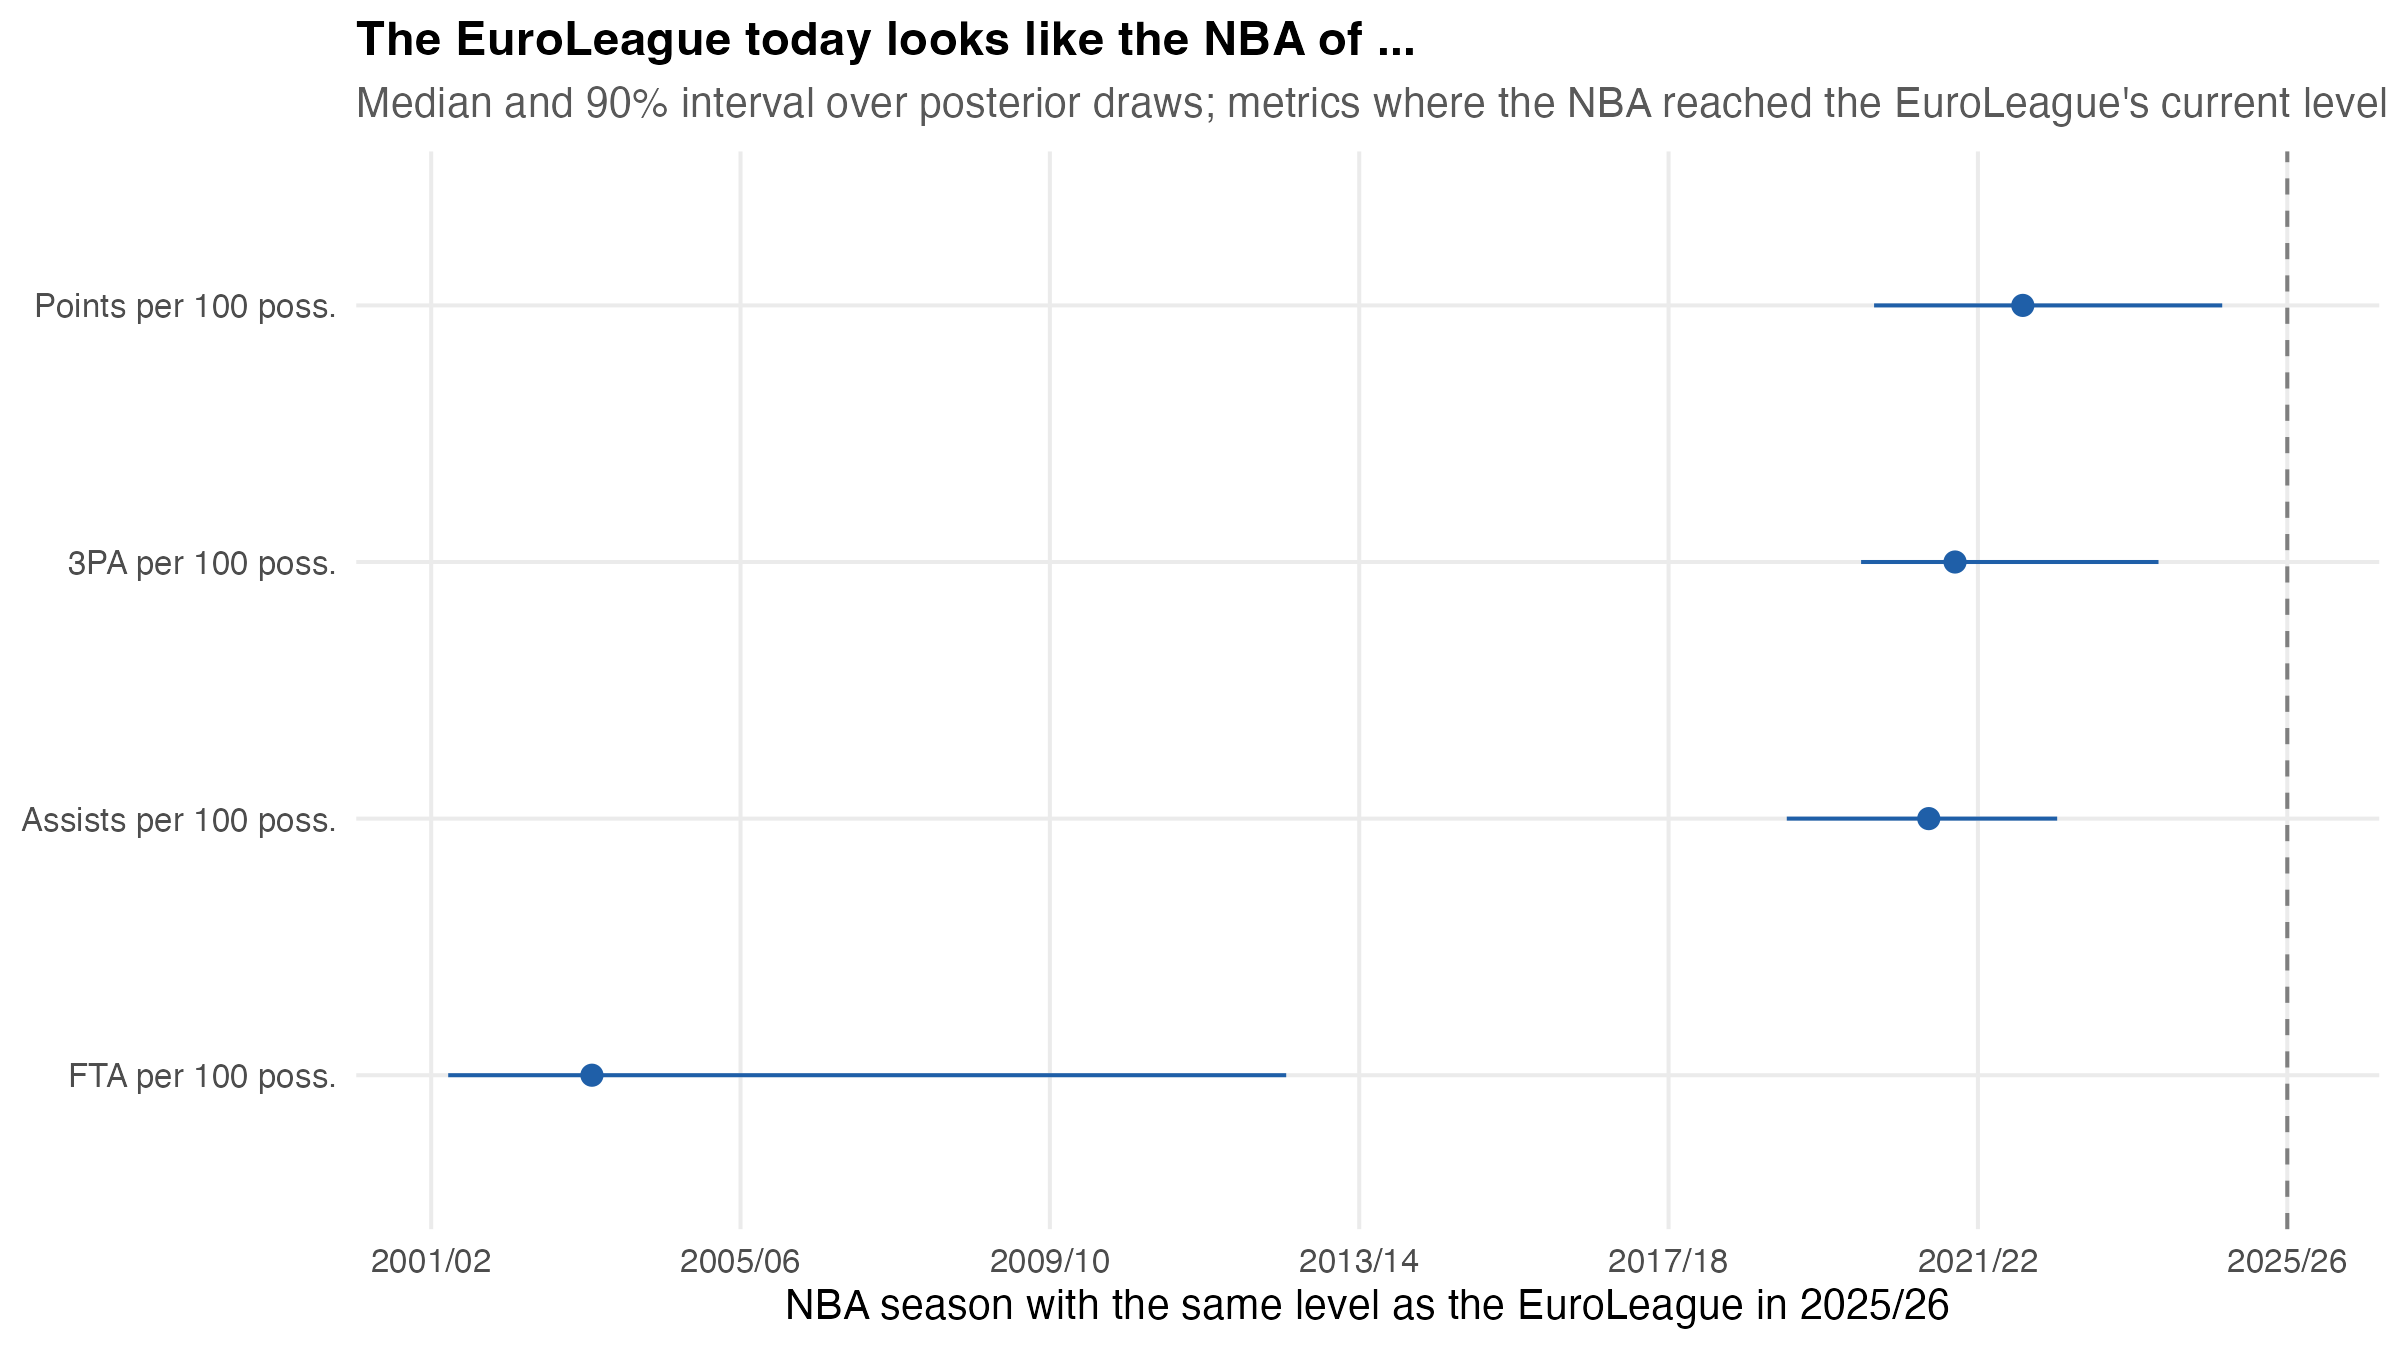
\includegraphics[width=0.85\textwidth,height=\textheight]{../RQ2_trends_leadlag/results/figures/fig4_time_gap.png}

}

\caption{\label{fig-timegap}The NBA season in which the NBA first
reached the EuroLeague's 2025/26 level (median and 90\% interval over
posterior draws), for metrics where it did.}

\end{figure}%

\subsection{The playoffs (RQ3)}\label{the-playoffs-rq3}

In the playoffs both leagues slow down, foul more, take more free throws
and shoot worse (Figure~\ref{fig-playoffs}). The NBA's playoff shift
points towards the EuroLeague's regular-season level on 10 of 21
metrics, mostly pace, fouls and free throws, and away from it on 8,
including every field-goal percentage (Figure~\ref{fig-toward}). The
2019 claim that NBA playoff basketball ``looks European'' therefore
holds for tempo and physicality but not for field-goal shooting. In shot
selection, EuroLeague teams swap rim shots for above-the-break threes in
the playoffs (-1.9 and +1.9 percentage points), while NBA teams move a
little from the rim to the short mid-range.

\begin{figure}[htbp]

\centering{

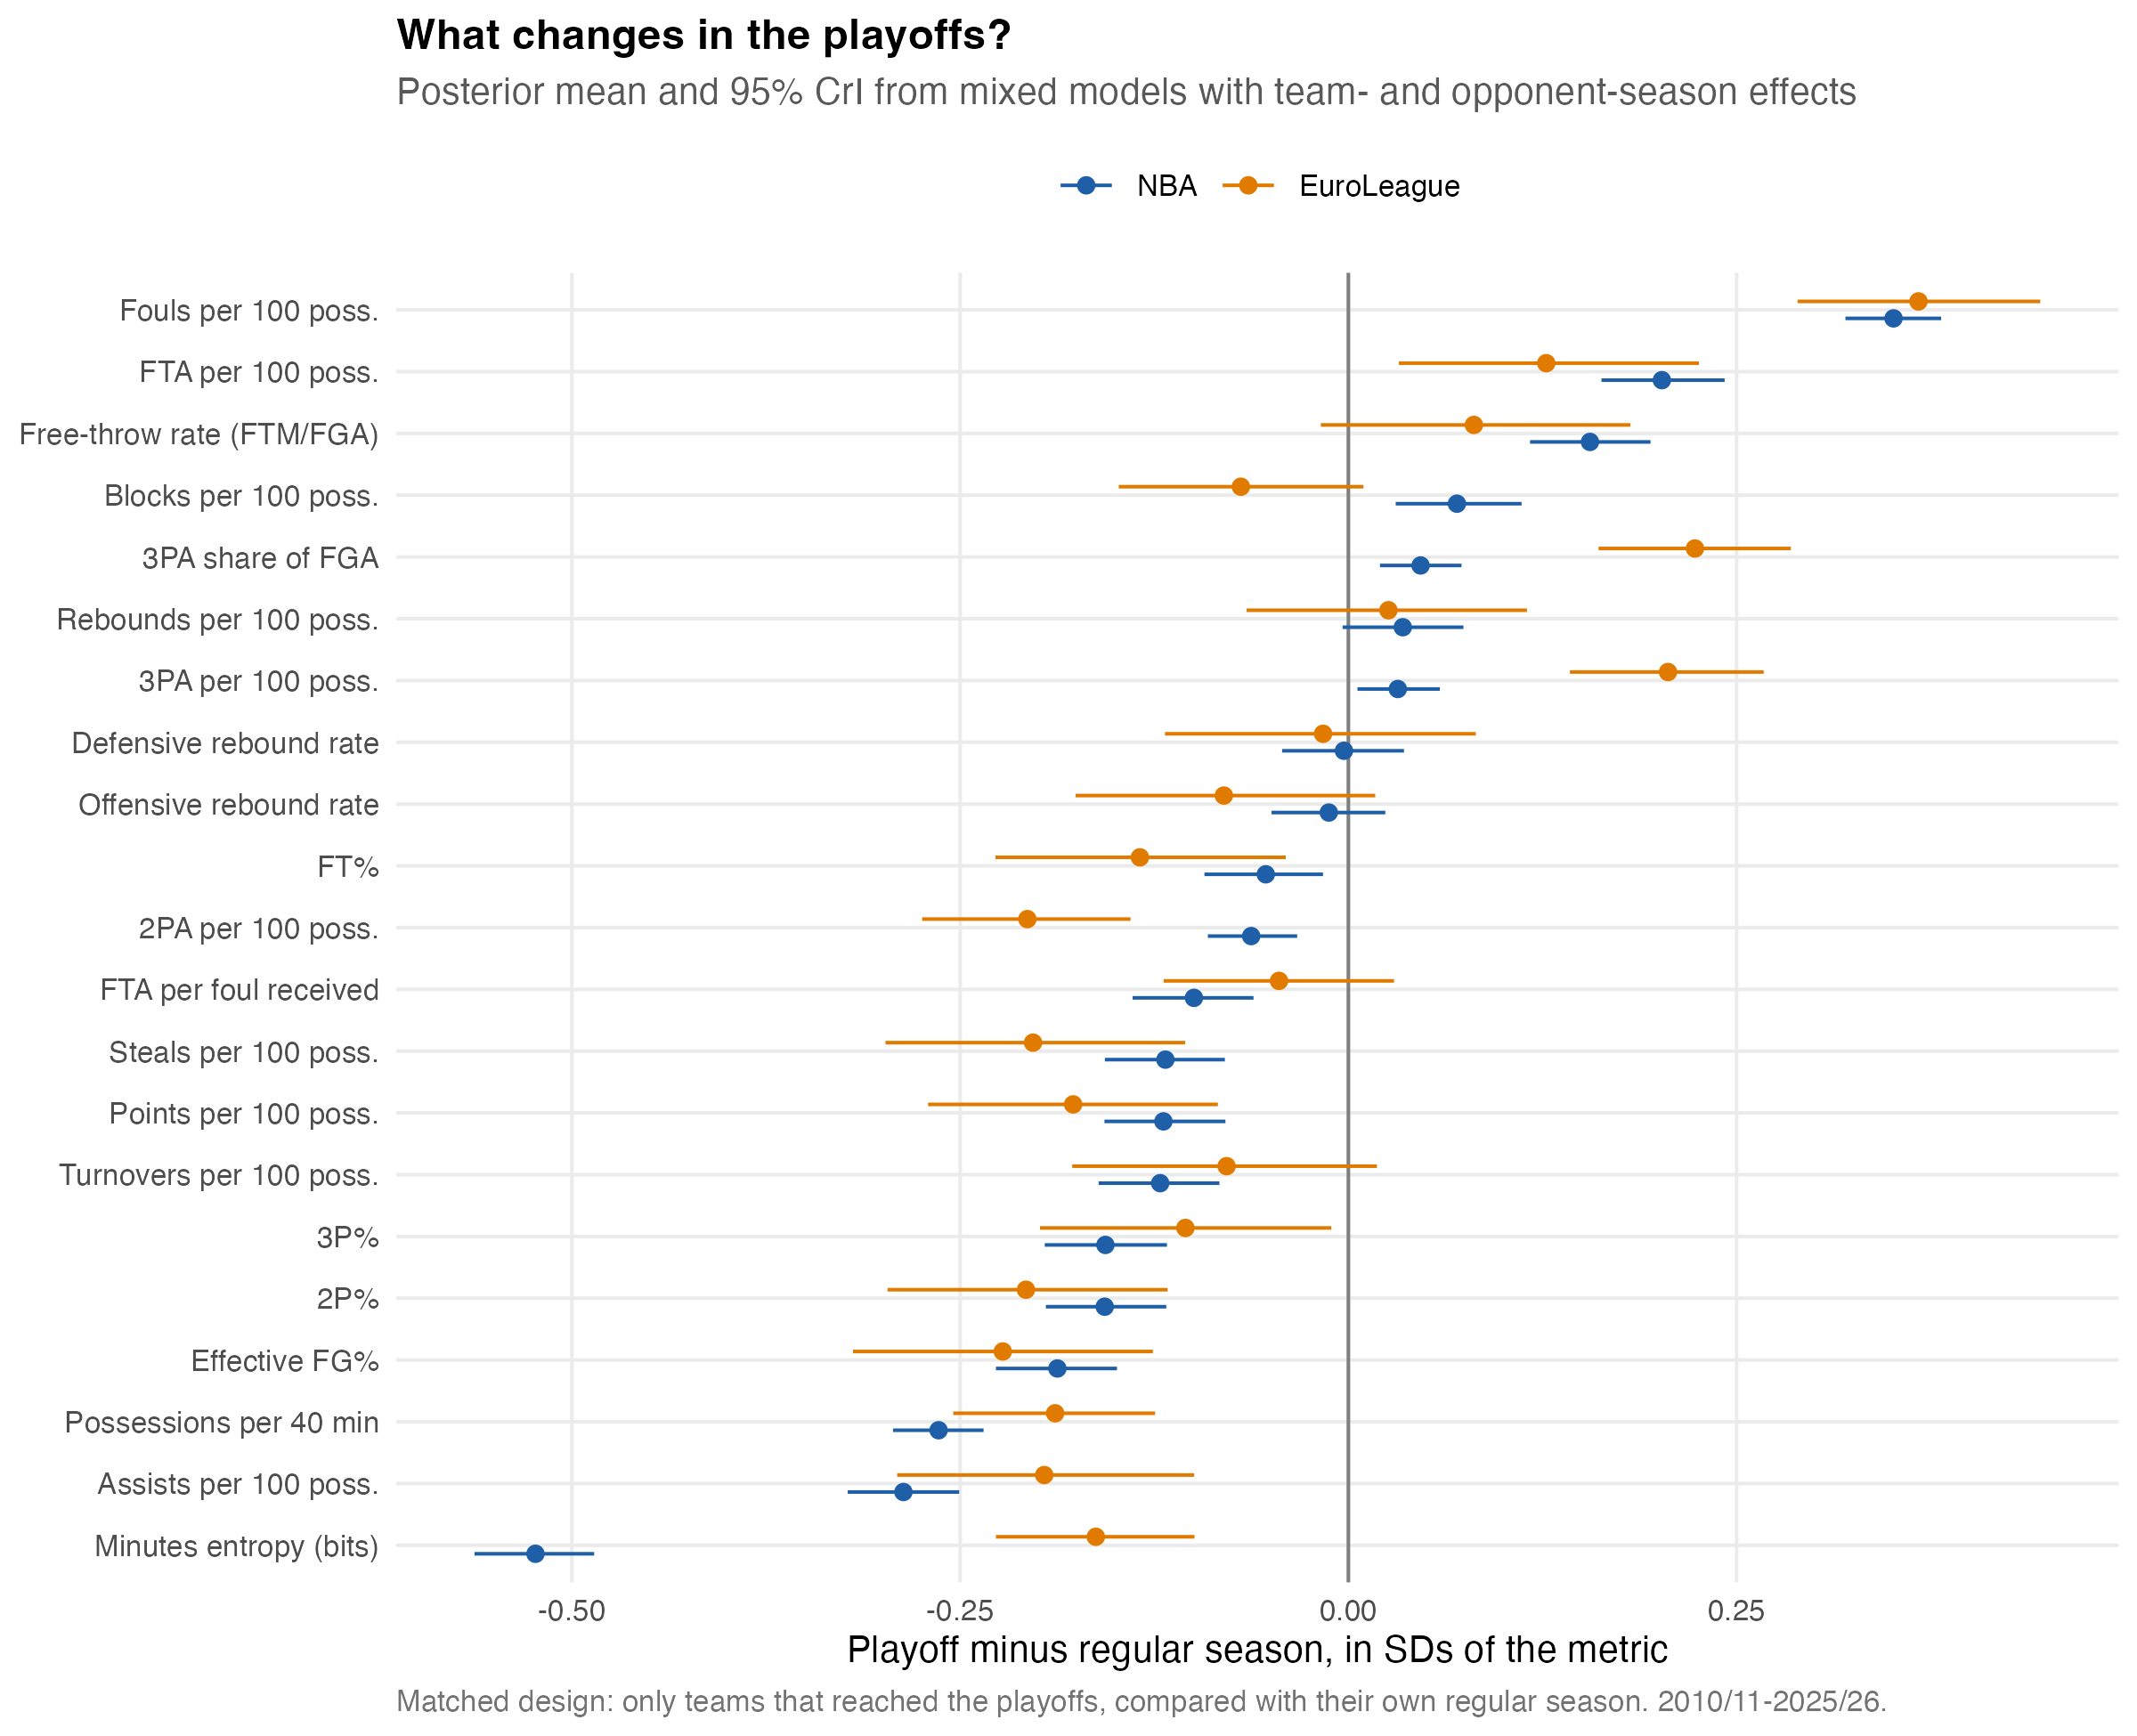
\includegraphics[width=0.85\textwidth,height=\textheight]{../RQ3_playoffs/results/figures/fig1_playoff_shifts.png}

}

\caption{\label{fig-playoffs}Playoff minus regular season for teams that
reached the playoffs, standardised; posterior means and 95\% credible
intervals, 2010/11--2025/26.}

\end{figure}%

\begin{figure}[htbp]

\centering{

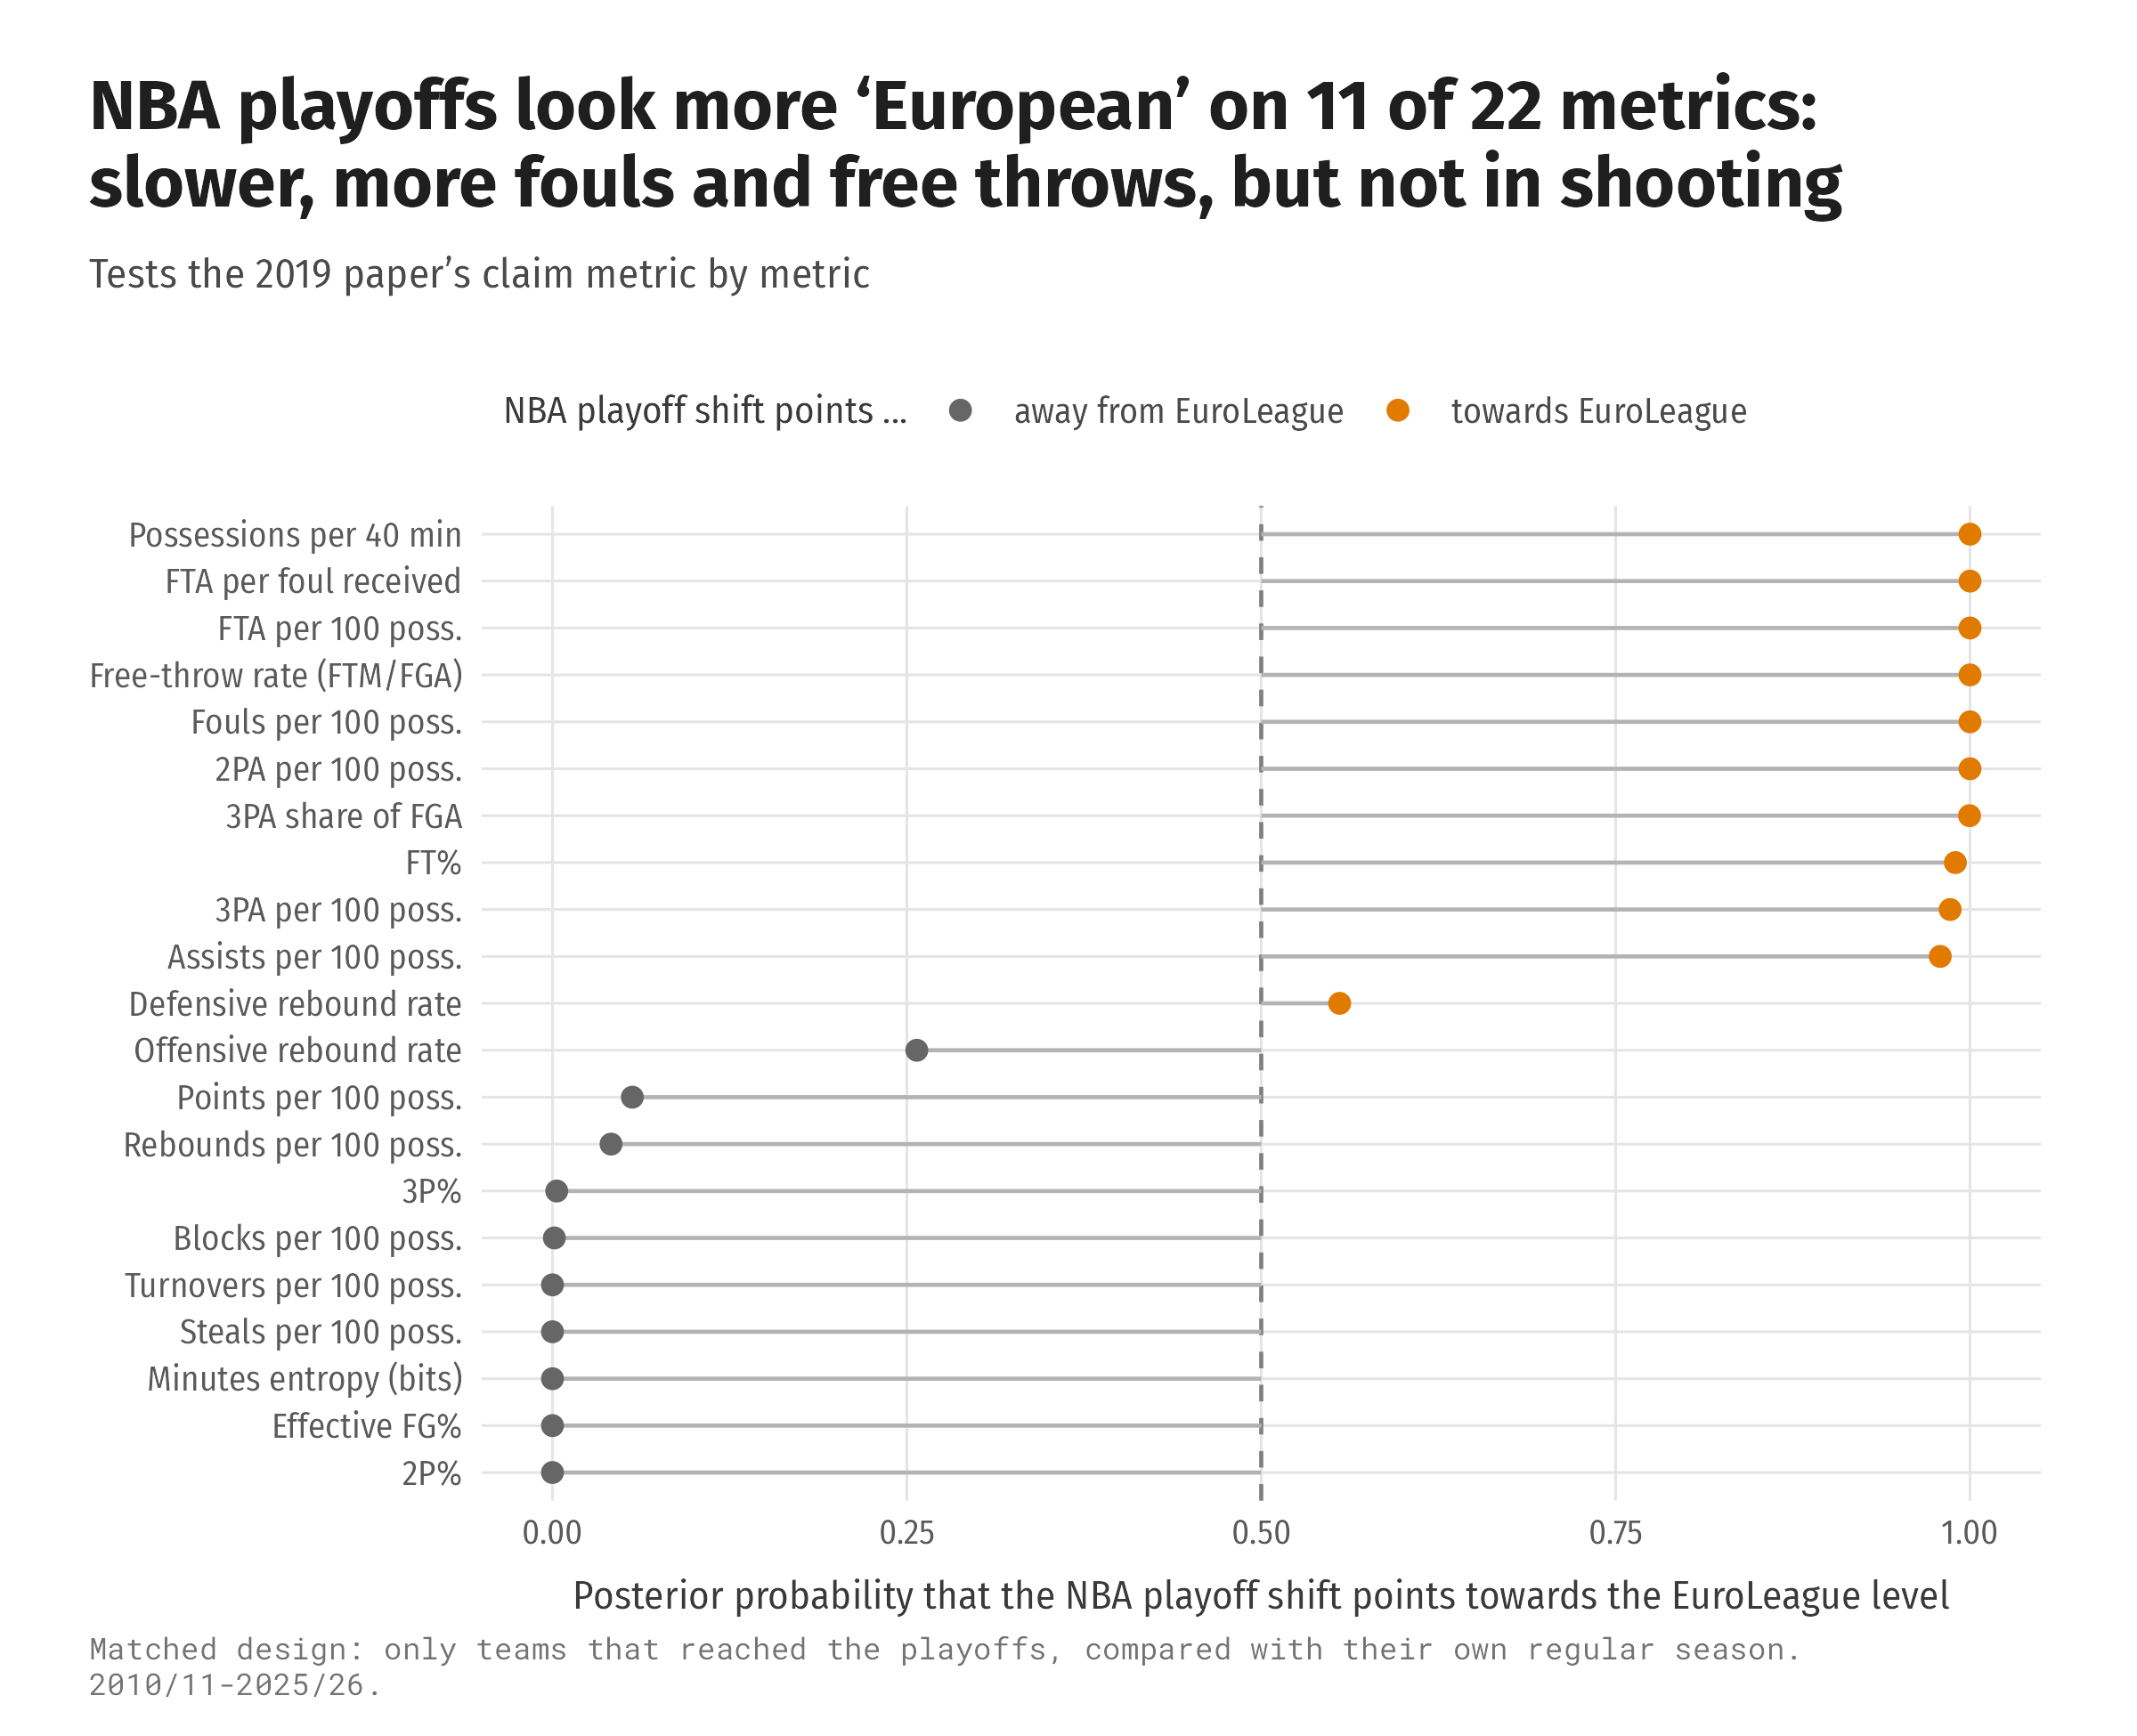
\includegraphics[width=0.85\textwidth,height=\textheight]{../RQ3_playoffs/results/figures/fig2_nba_toward_euroleague.png}

}

\caption{\label{fig-toward}Does the NBA's playoff shift point towards
the EuroLeague? Metric by metric.}

\end{figure}%

\subsection{Teams and players ahead of their time
(RQ4)}\label{teams-and-players-ahead-of-their-time-rq4}

The Houston Rockets were the NBA's most different team in seven straight
seasons (2013/14--2019/20): almost no long two-pointers, many corner
threes and free throws (Figure~\ref{fig-outliers}). Their 2012/13 and
2016/17 teams sit about four seasons ahead of the league, which later
moved their way (Figure~\ref{fig-timemachine}). In the EuroLeague, Real
Madrid of 2013/14--2017/18 played the league's future: fast,
assist-heavy, with few turnovers, almost no long two-pointers and many
above-the-break threes. Teams behind their time include the 2022/23
Chicago Bulls, whose mid-range offence resembled an NBA team of about
2017/18, and Partizan 2022/23.

\begin{figure}[htbp]

\centering{

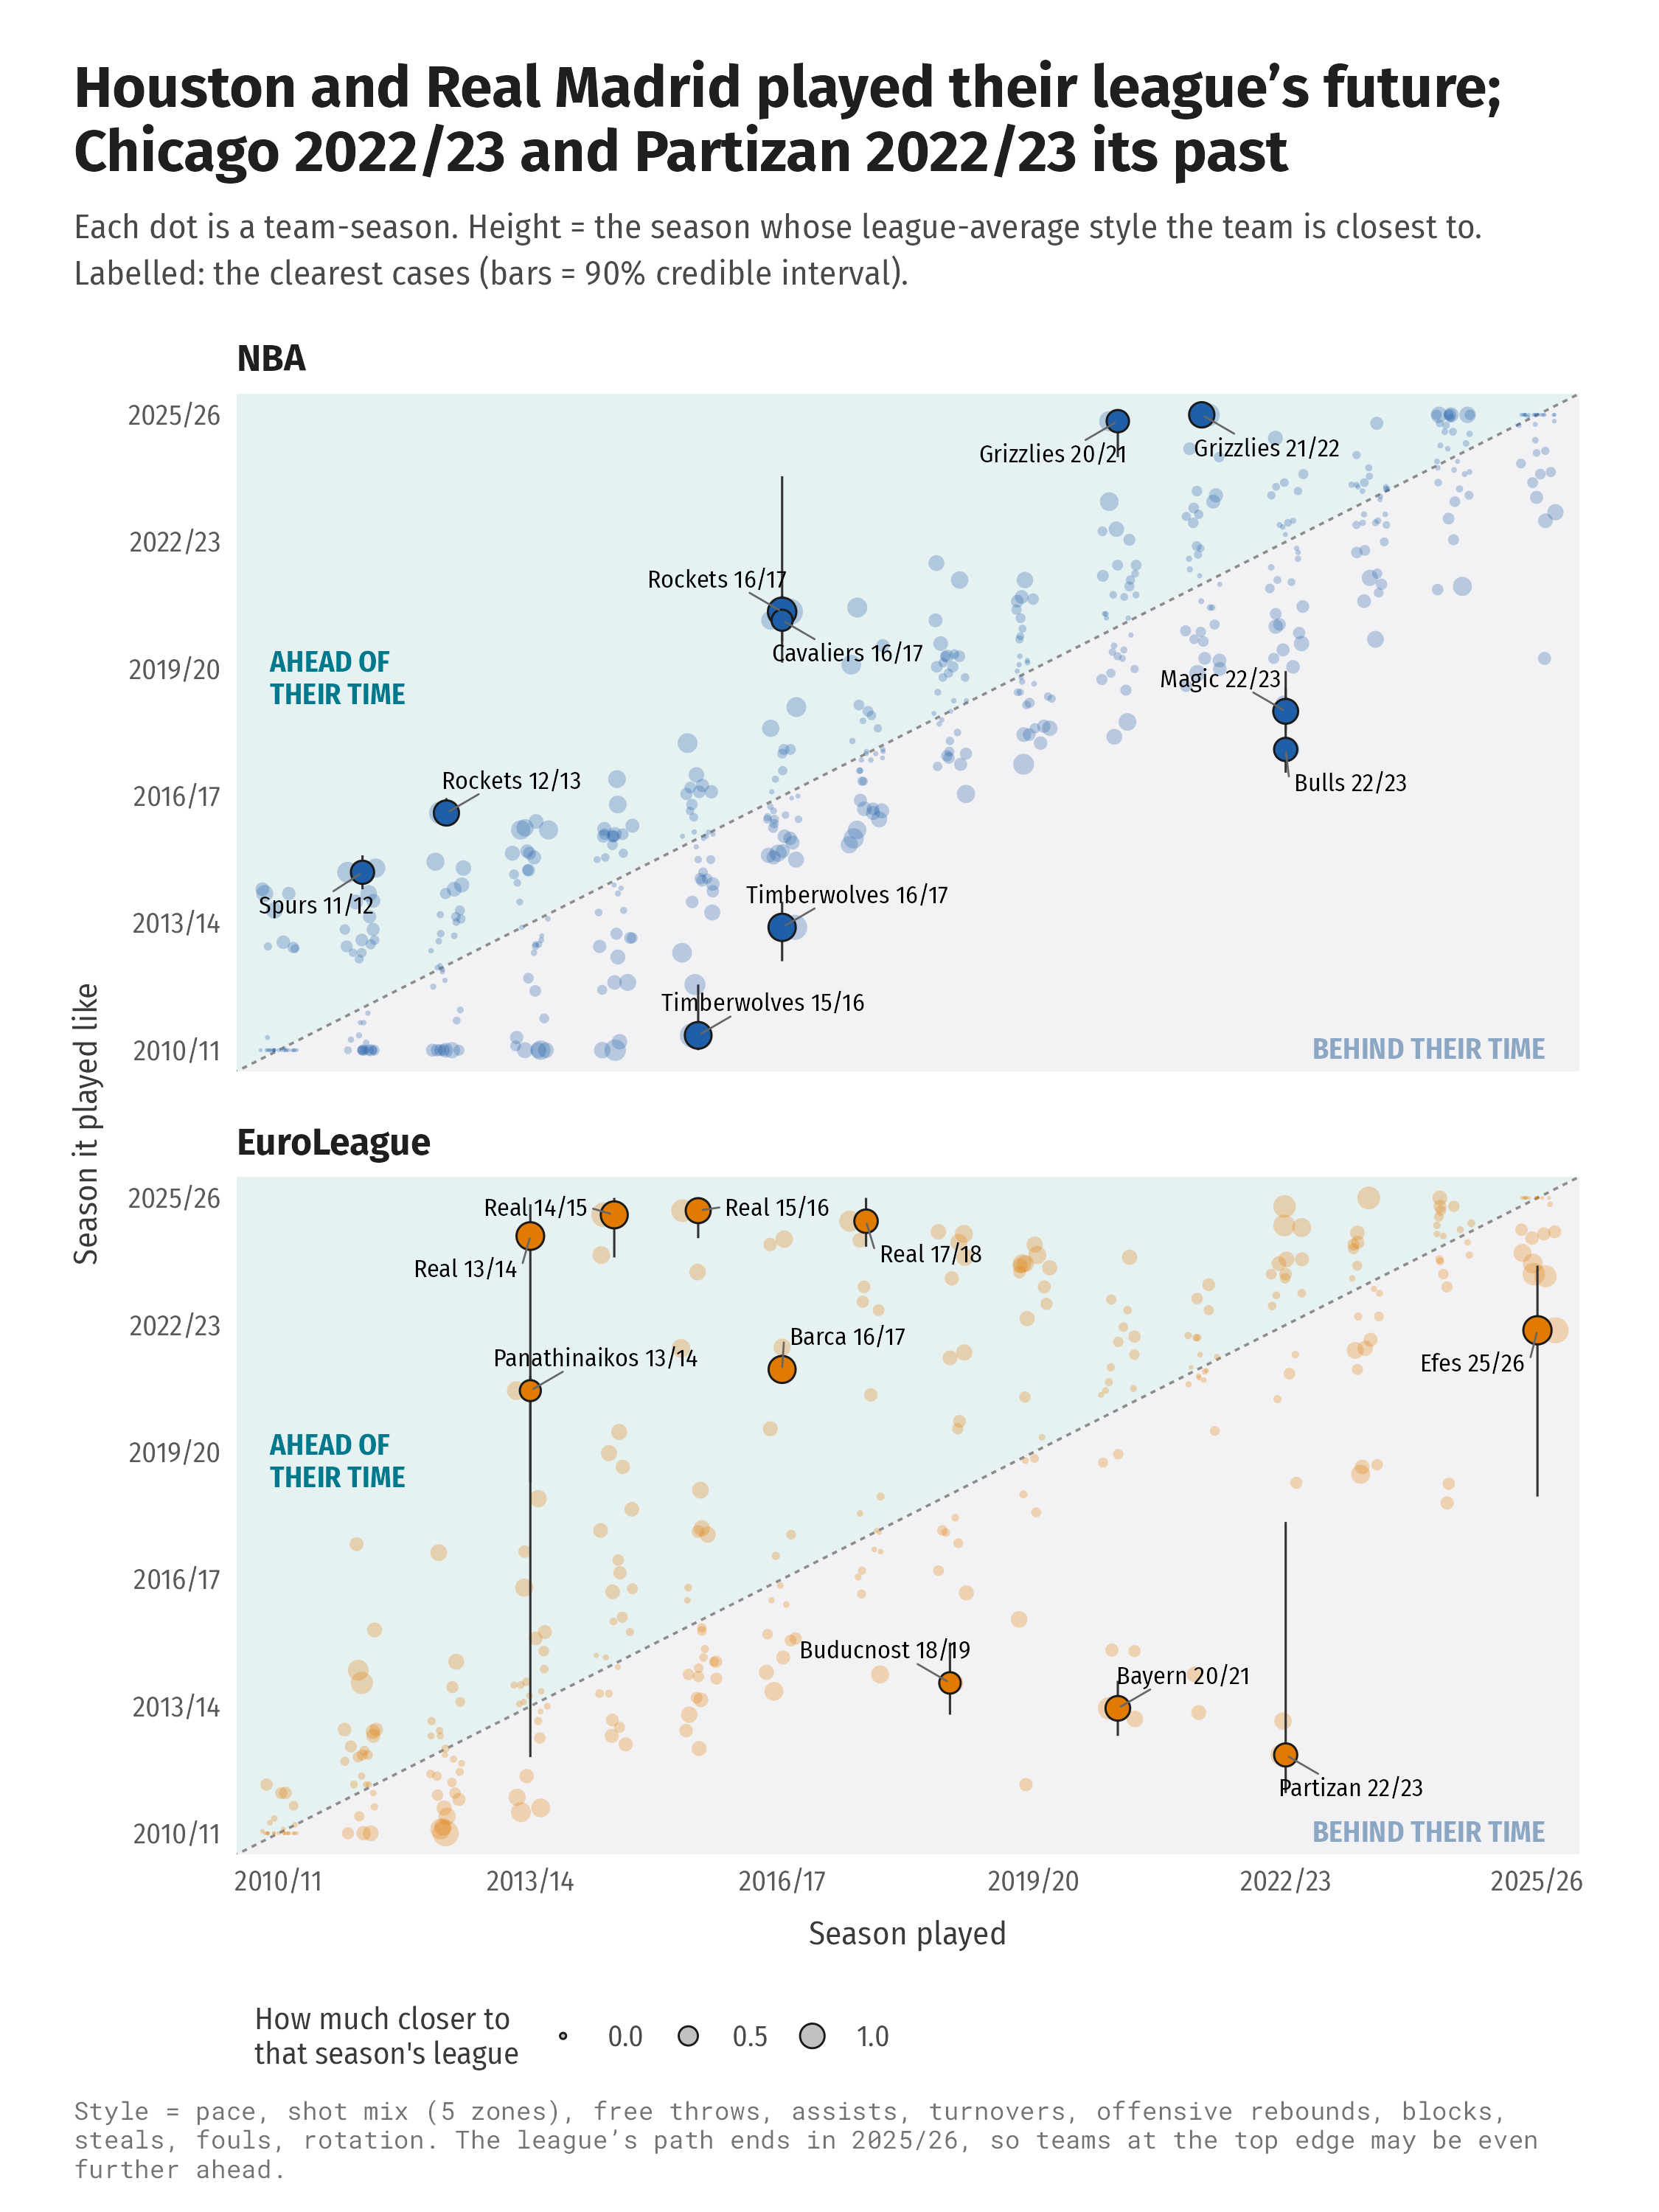
\includegraphics[width=11in,height=\textheight]{../RQ4_ahead_of_their_time/results/figures/fig1_time_machine_teams.png}

}

\caption{\label{fig-timemachine}The time machine: the season whose
league-average style each team-season is closest to. Above the diagonal
= ahead of its time; labelled teams are the clearest cases (bars = 90\%
credible intervals).}

\end{figure}%

\begin{figure}[htbp]

\centering{

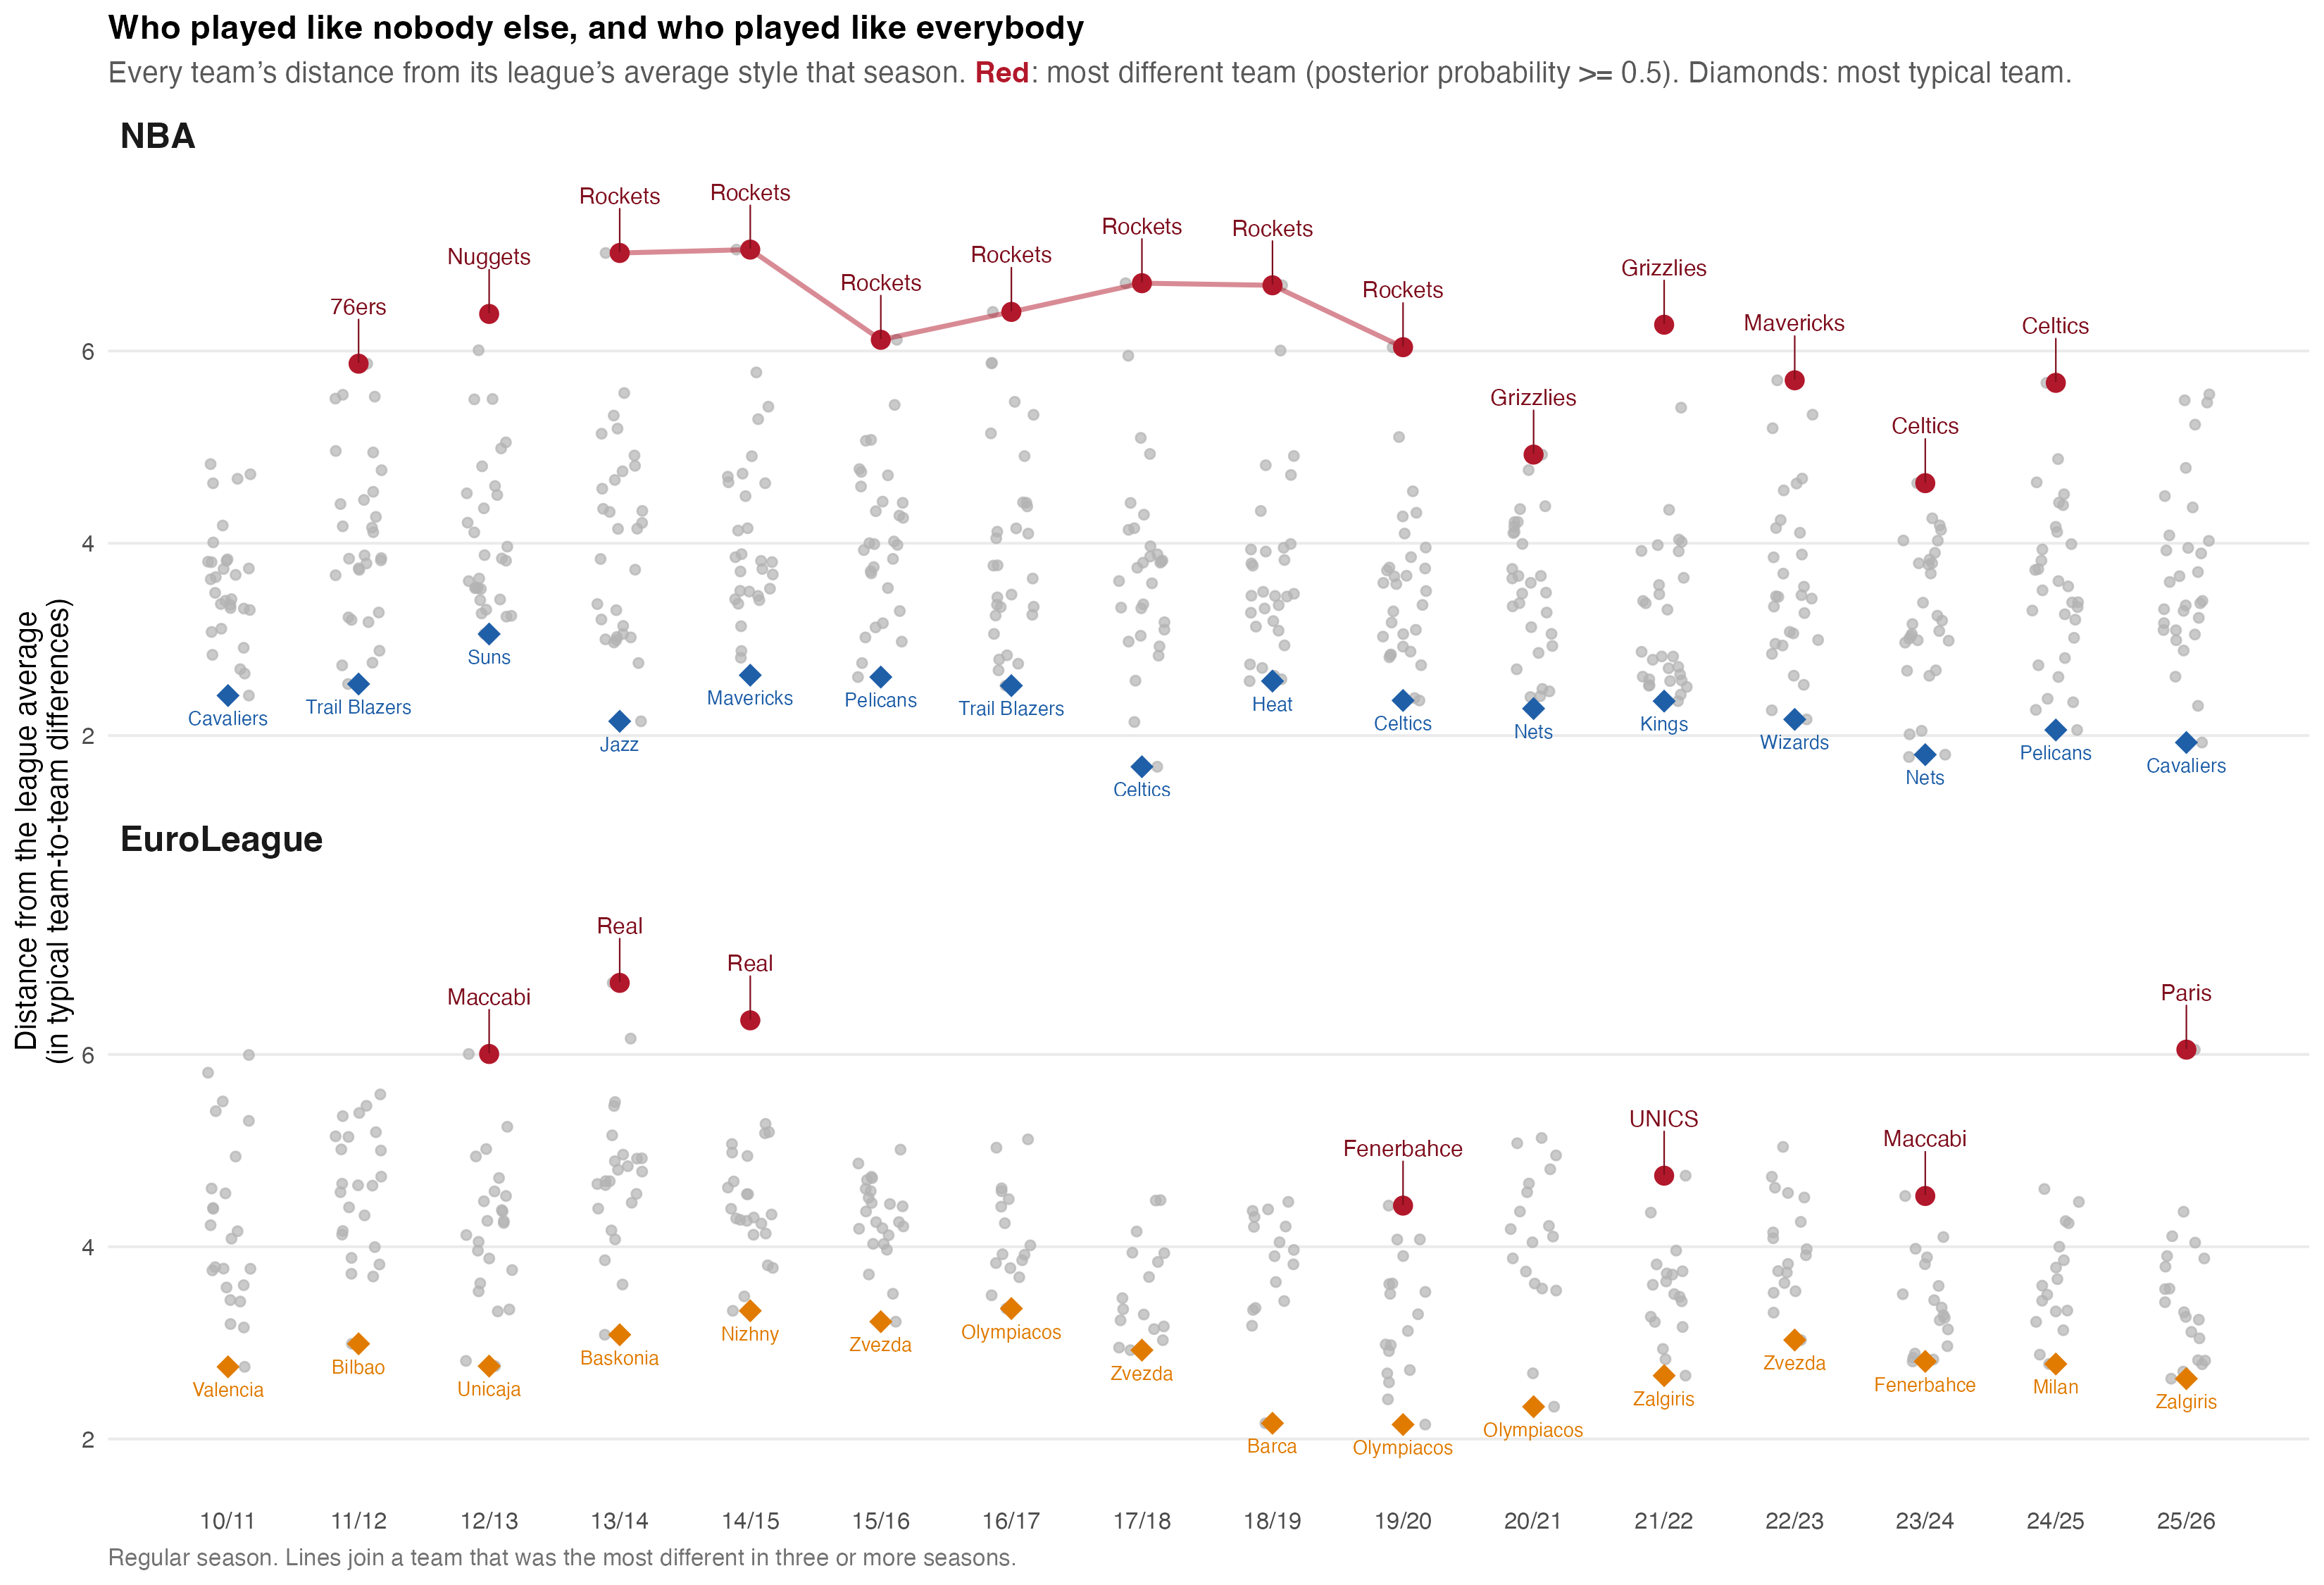
\includegraphics[width=11in,height=\textheight]{../RQ4_ahead_of_their_time/results/figures/fig2_outlier_teams.png}

}

\caption{\label{fig-outliers}Each team's distance from its league's
average style per season; red = the most different team of the season.}

\end{figure}%

Among players, Nikola Kalinić was the EuroLeague's most typical player
in six seasons. Brook Lopez is the clearest individual case of a player
jumping ahead: from 14 three-point attempts in 2015/16 to 387 in
2016/17, moving from a 2010s centre to a centre of today in one summer,
while his twin Robin stayed a 2010s centre (Figure~\ref{fig-lopez}).
EuroLeague guards such as Juan Carlos Navarro, Miloš Teodosić, Sergio
Llull and Vassilis Spanoulis sit ahead of their time for most of their
careers.

\begin{figure}[htbp]

\centering{

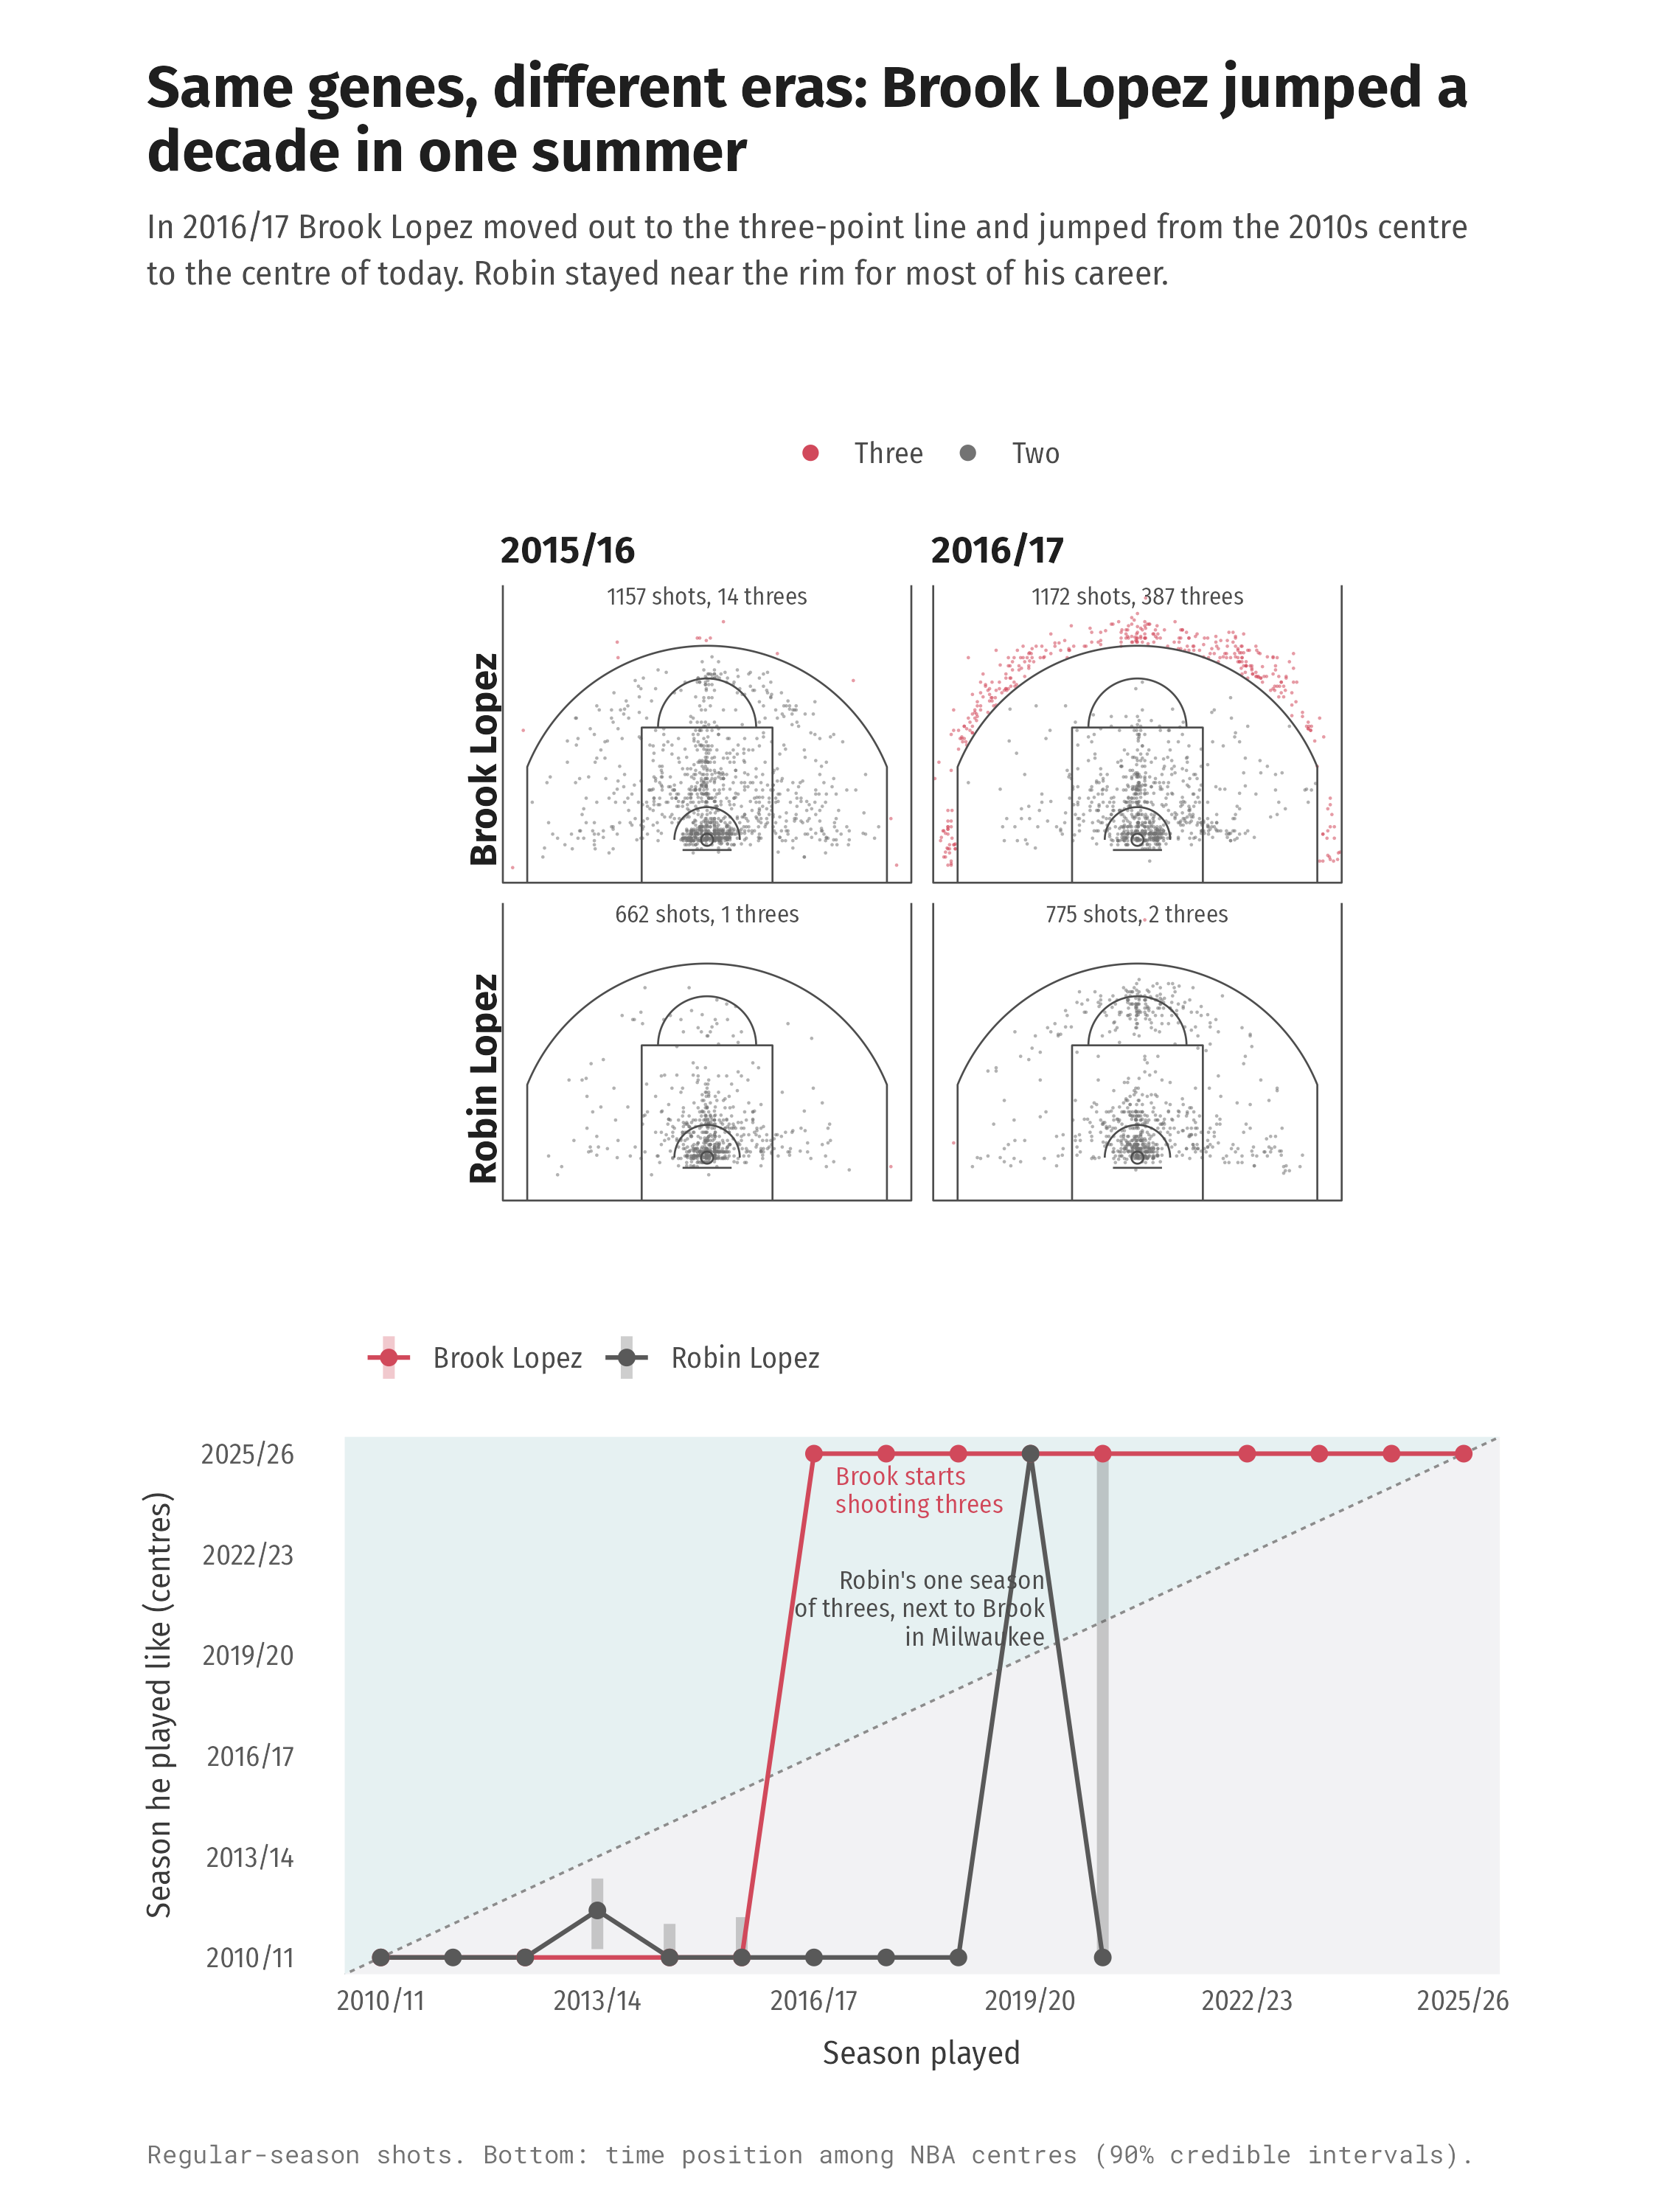
\includegraphics[width=12in,height=\textheight]{../RQ4_ahead_of_their_time/results/figures/fig4_lopez_twins.png}

}

\caption{\label{fig-lopez}Brook and Robin Lopez: shot charts before and
after 2016/17, and their time positions among NBA centres (90\% credible
intervals).}

\end{figure}%

\section{Discussion}\label{discussion}

Sixteen seasons on, the picture of Mandić et al. (2019) needs two
corrections. First, convergence is real but partial: the leagues now
shoot alike and take the same share of their shots from three, but they
have drifted apart in tempo and in how games are refereed. The NBA plays
about ten more possessions per 40 minutes and the EuroLeague commits
about seven more fouls per 100 possessions. Second, the idea that the
NBA ``became European'' is better described as two leagues responding to
the same pressures with different constraints. The EuroLeague took a
larger share of its threes earlier, but the NBA takes more threes per
possession, because it has more possessions and fewer turnovers. The
equal three-point share is reached from different spots on the floor,
shaped by the corner geometry of each court.

The lead--lag results describe timing, not influence. Smooth trends over
about 25 seasons can often be shifted a few seasons either way and still
fit, so for most metrics the honest answer is that the data cannot tell
who leads. Where they can, the EuroLeague moves with the NBA or one
season behind on three-point shooting, and resembles the NBA of three to
five seasons ago on volume measures.

\section{Limitations}\label{limitations}

Box scores and shot locations come from two scorekeeping systems: shots
near the rim are recorded less precisely in the EuroLeague, and rebounds
and turnovers are credited slightly differently. The EuroLeague's format
changed several times (Top 16 until 2015/16, a single round robin since
2016/17, a play-in since 2025/26), and the 2019/20 season was cancelled
after the regular season. Lead--lag results describe timing only; shared
causes such as analytics, rule changes and player movement could produce
the same pattern. The RQ4 results depend on which features define style;
a different list could name different teams or players, and the
posterior probabilities show where the choice is close. NBA possessions
per 40 minutes before 2010/11 use regulation length, which only affects
the lead--lag model.

\section{Data and code availability}\label{data-and-code-availability}

All code, Stan models, result tables and figures are at
\url{https://github.com/loukesio/nba-vs-euroleague} (MIT licence). The
data are downloaded from public sources by the scripts in
\texttt{00\_data/scripts/} and remain subject to their providers' terms.
Figures were made with ggbasket
(\url{https://loukesio.github.io/ggbasket/}).

\section*{References}\label{references}
\addcontentsline{toc}{section}{References}

\phantomsection\label{refs}
\begin{CSLReferences}{1}{0}
\bibitem[\citeproctext]{ref-burkner2017}
Bürkner, Paul-Christian. 2017. {``Brms: An {R} Package for {Bayesian}
Multilevel Models Using {Stan}.''} \emph{Journal of Statistical
Software} 80 (1): 1--28. \url{https://doi.org/10.18637/jss.v080.i01}.

\bibitem[\citeproctext]{ref-carpenter2017}
Carpenter, Bob, Andrew Gelman, Matthew D. Hoffman, Daniel Lee, Ben
Goodrich, Michael Betancourt, Marcus Brubaker, Jiqiang Guo, Peter Li,
and Allen Riddell. 2017. {``Stan: A Probabilistic Programming
Language.''} \emph{Journal of Statistical Software} 76 (1): 1--32.
\url{https://doi.org/10.18637/jss.v076.i01}.

\bibitem[\citeproctext]{ref-erculj2015}
Erčulj, Frane, and Erik Štrumbelj. 2015. {``Basketball Shot Types and
Shot Success in Different Levels of Competitive Basketball.''}
\emph{PLOS ONE} 10 (6): e0128885.
\url{https://doi.org/10.1371/journal.pone.0128885}.

\bibitem[\citeproctext]{ref-hoopr}
Gilani, Saiem. 2021. \emph{{hoopR}: Access Men's Basketball Play by Play
Data}. \url{https://hoopr.sportsdataverse.org}.

\bibitem[\citeproctext]{ref-goldsberry2019}
Goldsberry, Kirk. 2019. \emph{SprawlBall: A Visual Tour of the New Era
of the {NBA}}. Boston: Houghton Mifflin Harcourt.

\bibitem[\citeproctext]{ref-kubatko2007}
Kubatko, Justin, Dean Oliver, Kevin Pelton, and Dan T. Rosenbaum. 2007.
{``A Starting Point for Analyzing Basketball Statistics.''}
\emph{Journal of Quantitative Analysis in Sports} 3 (3).
\url{https://doi.org/10.2202/1559-0410.1070}.

\bibitem[\citeproctext]{ref-mandic2019}
Mandić, Radivoj, Saša Jakovljević, Frane Erčulj, and Erik Štrumbelj.
2019. {``Trends in {NBA} and {Euroleague} Basketball: Analysis and
Comparison of Statistical Data from 2000 to 2017.''} \emph{PLOS ONE} 14
(10): e0223524. \url{https://doi.org/10.1371/journal.pone.0223524}.

\bibitem[\citeproctext]{ref-oliver2004}
Oliver, Dean. 2004. \emph{Basketball on Paper: Rules and Tools for
Performance Analysis}. Washington, DC: Potomac Books.

\bibitem[\citeproctext]{ref-rue2005}
Rue, Håvard, and Leonhard Held. 2005. \emph{Gaussian Markov Random
Fields: Theory and Applications}. Boca Raton, FL: Chapman; Hall/CRC.

\bibitem[\citeproctext]{ref-ggbasket}
Theodosiou, Loukas. 2026. \emph{{ggbasket}: Learn from Basketball Games,
{NBA} and {EuroLeague}}. \url{https://loukesio.github.io/ggbasket/}.

\bibitem[\citeproctext]{ref-wood2017}
Wood, Simon N. 2017. \emph{Generalized Additive Models: An Introduction
with {R}}. 2nd ed. Boca Raton, FL: Chapman; Hall/CRC.

\end{CSLReferences}



\end{document}
